\documentclass[11pt]{article}

\usepackage[T1]{fontenc}
\usepackage[utf8]{inputenc}
\usepackage[provide=*,spanish]{babel}
\usepackage{lmodern}
\usepackage{microtype}
\usepackage[margin=1in]{geometry}
\usepackage{amsmath}
\usepackage{amssymb}
\usepackage{graphicx}
\usepackage{booktabs}
\usepackage{tabularx}
\usepackage{longtable}
\usepackage{array}
\usepackage{url}
\usepackage{cite}
\usepackage{xcolor}
\usepackage[colorlinks=true,linkcolor=blue,citecolor=blue,urlcolor=blue]{hyperref}
\definecolor{docnotelinkcolor}{rgb}{0,0,0.65}

\graphicspath{{../figures/}}

\title{Evaluación de la Fiabilidad de Reconocimiento de Conjunto Abierto en la Clasificación Morfológica de Leucocitos bajo Cambio de Dominio}
\author{G. Álvarez Sánchez}
\date{}

\begin{document}
\maketitle

\begin{abstract}
Los clasificadores automatizados de morfología leucocitaria suelen evaluarse bajo el supuesto de conjunto cerrado, aunque los modelos desplegados o reutilizados pueden encontrar morfologías fuera de la taxonomía de entrenamiento. Evaluamos si un alto rendimiento de conjunto cerrado implica un rechazo fiable de morfologías no vistas bajo cambio de dominio interno y externo. La taxonomía conocida incluyó basófilos, eosinófilos, linfocitos, monocitos y neutrófilos segmentados. En MLL23 se usaron 12,793 imágenes conocidas para entrenamiento, 2,741 para validación, 2,742 para prueba conocida y 23,345 imágenes retenidas de 13 morfologías para prueba desconocida. Se evaluaron modelos ResNet18 preentrenados en ImageNet, entrenados con entropía cruzada o ArcFace, en cinco semillas y dos protocolos de partición mediante puntuaciones post hoc de conjunto abierto. El rendimiento interno de conjunto cerrado fue alto para ambas pérdidas, con macro-F1 aproximado de 0.97. El reconocimiento interno de conjunto abierto fue menor: CE+ViM alcanzó AUROC 0.877 $\pm$ 0.004 en V1 y 0.874 $\pm$ 0.008 en la partición de sensibilidad V2 consciente de casi duplicados, con FPR@95TPR 0.484 $\pm$ 0.027 y 0.528 $\pm$ 0.050. En AML-Cytomorphology\_LMU, un conjunto independiente de 18,365 imágenes usado solo para prueba, el rendimiento se degradó sustancialmente; el AUROC externo varió de 0.563 a 0.696 en sistemas V1 y de 0.573 a 0.696 en sistemas V2, con FPR@95TPR alto. El fallo dependió de la morfología, con neutrophil-band, monoblast, myeloblast y atypical lymphocyte entre los desconocidos externos más difíciles. ArcFace mejoró algunos resúmenes geométricos de clases conocidas, pero no se reprodujo como una representación superior robusta para conjunto abierto. Los análisis de homología persistente fueron negativos o explicativos, no predictivos. Por tanto, una clasificación leucocitaria fuerte de conjunto cerrado no aseguró un rechazo fiable de morfologías no vistas, especialmente bajo similitud morfológica y cambio de dominio externo.
\end{abstract}

\noindent\textbf{Palabras clave:} reconocimiento de conjunto abierto; morfología leucocitaria; cambio de dominio; detección fuera de distribución; análisis de imágenes hematológicas; validación externa

\section{Introducción}

La morfología microscópica de leucocitos sigue siendo una fuente central de información en hematología. La revisión experta de frotis de sangre periférica y médula ósea apoya recuentos diferenciales, control de calidad de analizadores automatizados y reconocimiento de morfologías que pueden requerir interpretación adicional de laboratorio. En paralelo, las redes neuronales convolucionales y métodos relacionados de análisis de imágenes han alcanzado alta exactitud en conjuntos curados de imágenes de células sanguíneas, incluidas colecciones de morfología de sangre periférica y médula ósea \cite{walter2023_ai_hematology,khan2021_wbc_review,deshpande2021_blood_cells_review,acevedo2019_peripheral_blood_cnn,matek2019_blast,matek2021_bone_marrow}. Estos avances hacen del reconocimiento automatizado de morfología un problema de investigación sólido para el análisis de imágenes biomédicas. También crean un riesgo metodológico: el rendimiento de conjunto cerrado puede parecer convincente aun cuando la evaluación nunca pregunta qué ocurre con células fuera de la taxonomía de entrenamiento.

El escenario convencional de conjunto cerrado asume que toda imagen de prueba pertenece a una de las clases vistas durante el entrenamiento. Esa suposición es conveniente para aprendizaje supervisado, pero es frágil para reconocimiento morfológico. Un modelo entrenado con categorías de leucocitos maduros puede encontrar células inmaduras, atípicas, raras, dañadas o fuera de taxonomía en tiempo de prueba. Si la evaluación fuerza cada imagen de ese tipo a una de las clases conocidas, el modelo puede parecer confiado mientras realiza la tarea equivocada. El reconocimiento de conjunto abierto aborda esta brecha al requerir que un sistema clasifique muestras conocidas y rechace muestras de clases no vistas \cite{scheirer2013_open_set,geng2021_osr_survey,bendale2016_openmax,yang2024_generalized_ood}. En este estudio, la pregunta de conjunto abierto es deliberadamente estrecha: ¿puede un clasificador entrenado en una taxonomía fija de morfología leucocitaria identificar que una imagen de prueba no debe asignarse a esa taxonomía?

Esta distinción es especialmente importante porque ``desconocido'' tiene aquí un significado técnico. Las clases conocidas son basophil, eosinophil, lymphocyte, monocyte y neutrophil\_segmented. Una muestra desconocida es una morfología fuera de esa taxonomía de entrenamiento. No es una etiqueta de cáncer, leucemia, malignidad, diagnóstico anormal, desenlace a nivel de paciente ni hallazgo clínicamente positivo. Por ello, el trabajo no debe leerse como un sistema diagnóstico ni como detector de leucemia. Es un estudio empírico de fiabilidad de reconocimiento cuando el inventario de etiquetas del modelo está incompleto.

Las muestras desconocidas más difíciles a menudo no son visualmente ajenas. Un neutrófilo en banda está cerca de los neutrófilos segmentados; un monoblasto puede ser atraído hacia monocitos; las morfologías blásticas o linfoides atípicas pueden parecerse al vecindario de linfocitos típicos. Tales ejemplos no son simplemente valores atípicos genéricos. Son morfologías cercanas a la taxonomía cuyos errores pueden estar estructurados por linaje celular, maduración, adquisición de imagen y geometría de representación. Esto convierte al reconocimiento leucocitario de conjunto abierto en un problema exigente de análisis de imágenes biomédicas: el modelo debe rechazar muestras relacionadas con las clases conocidas, pero no miembros de ellas.

El cambio de dominio externo agrava el problema. Los conjuntos de imágenes hematológicas pueden diferir en tinción, escáner, objetivo, recorte, política de anotación, mezcla de pacientes, tamaño de imagen y composición de clases. Trabajos previos en análisis de imágenes médicas y clasificación de células sanguíneas han mostrado que los modelos entrenados y probados bajo condiciones de imagen similares pueden perder rendimiento al evaluarse entre fuentes \cite{guan2022_domain_adaptation_medical,litjens2017_medical_ai_survey,salehi2022_cross_domain,sadafi2024_continual_wbc,tsutsui2023_wbc_domain_shift}. Para reconocimiento de conjunto abierto, la validación externa es aún más exigente porque pueden cambiar simultáneamente la clasificación de clases conocidas y el rechazo de desconocidos. Una puntuación estable internamente puede dejar de ordenar correctamente los métodos en un nuevo dominio de adquisición.

A pesar del trabajo extenso en clasificación leucocitaria y del crecimiento en reconocimiento de conjunto abierto y detección fuera de distribución, la evidencia sigue siendo limitada para protocolos que retienen explícitamente morfologías hematológicas nombradas como clases desconocidas, evalúan múltiples semillas, preservan los desconocidos como datos solo de prueba y examinan si los rankings internos se transfieren a un conjunto hematológico externo. Esta brecha motiva el presente manuscrito. Evaluamos un protocolo congelado de conjunto abierto usando MLL23 como dominio interno y AML-Cytomorphology\_LMU como dominio independiente solo de prueba \cite{mll23_nature_2025,mll23_zenodo_2024,aml_lmu_tcia_2019}. La tesis científica es que un alto rendimiento de clasificación de conjunto cerrado en morfología leucocitaria no implica reconocimiento fiable de conjunto abierto de morfologías no vistas, en particular bajo similitud morfológica y cambio de dominio externo.

Las contribuciones son:
\begin{itemize}
\item Un protocolo reproducible de evaluación de conjunto abierto para reconocimiento de morfología leucocitaria, con una taxonomía conocida congelada de cinco clases y morfologías de MLL23 retenidas usadas solo para prueba de conjunto abierto.
\item Un análisis de sensibilidad de cinco semillas y dos particiones que muestra que macro-F1 interno de conjunto cerrado cercano a 0.97 coexiste con rechazo imperfecto de desconocidos y FPR@95TPR alto.
\item Una validación externa solo de prueba en AML-Cytomorphology\_LMU que muestra degradación sustancial por cambio de dominio e inestabilidad de rankings metodológicos internos.
\item Un análisis de fallos por morfología que muestra que el rechazo difícil de desconocidos está estructurado por atractores de clases conocidas como banda-a-neutrófilo segmentado, monoblasto-a-monocito y linfoide-a-linfocito.
\item Evidencia negativa o secundaria controlada que muestra que una mejor geometría de clases conocidas y los descriptores de homología persistente no se traducen automáticamente en reconocimiento robusto de conjunto abierto.
\end{itemize}

\begin{figure}[htbp]
\centering
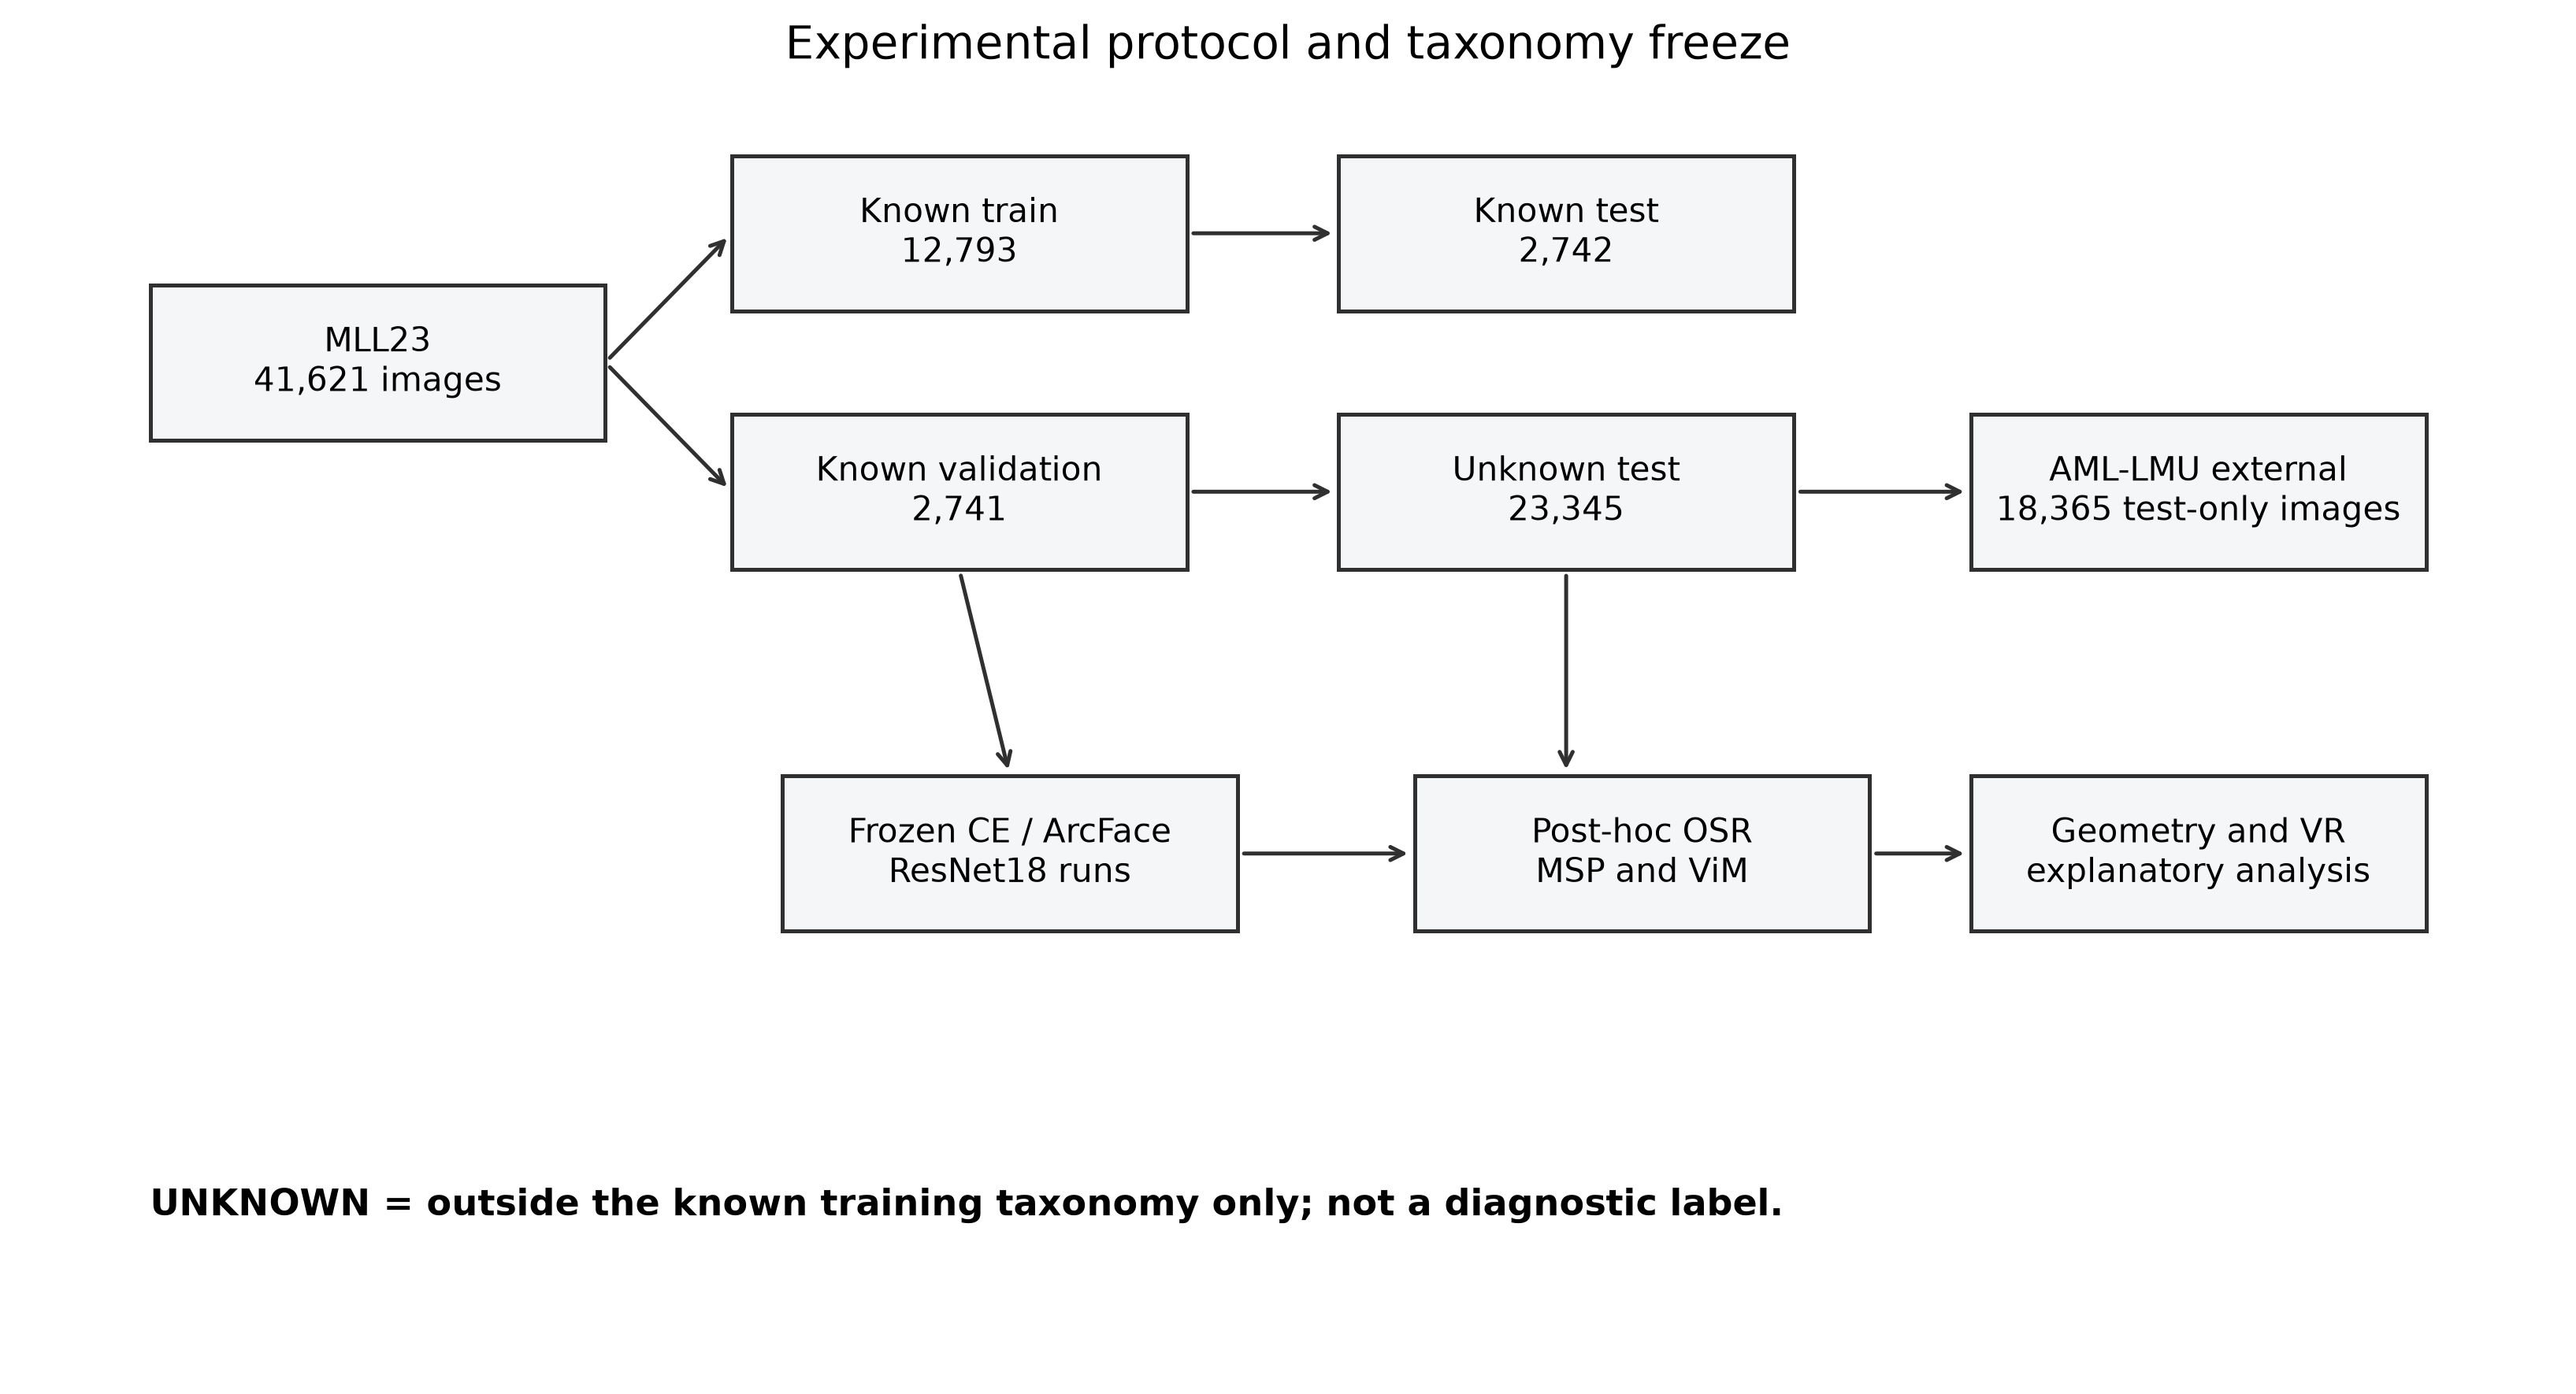
\includegraphics[width=\textwidth]{figure1_protocol.png}
\caption{Protocolo congelado de evaluación de conjunto abierto. MLL23 se usa para evaluación interna multisemilla, con cinco clases de leucocitos maduros tratadas como conocidas y 13 morfologías retenidas como desconocidas. AML-Cytomorphology\_LMU se usa solo como dominio externo de prueba, sin entrenamiento, ajuste, calibración ni ajuste de representación.}
\label{fig:protocol}
\end{figure}

\section{Trabajo Relacionado}

\subsection{Clasificación Automatizada de Morfología Leucocitaria}

El análisis automatizado de imágenes de células sanguíneas tiene una larga historia, pero el progreso reciente ha sido impulsado por conjuntos anotados de células individuales y redes neuronales convolucionales. Las revisiones de clasificación de glóbulos blancos reportan una literatura amplia sobre segmentación, extracción de características, aprendizaje por transferencia y clasificadores profundos para imágenes microscópicas de frotis sanguíneos \cite{khan2021_wbc_review,deshpande2021_blood_cells_review}. Gran parte de este trabajo evalúa un conjunto fijo de clases y reporta exactitud, precisión, exhaustividad o F1 bajo particiones del mismo conjunto de datos. Tales estudios son útiles para establecer factibilidad de clasificación, pero en general no prueban si un modelo puede rechazar una muestra fuera de su inventario de etiquetas.

Varios estudios influyentes de análisis de imágenes hematológicas demuestran la fuerza del aprendizaje profundo en escenarios de conjunto cerrado o tareas específicas. Acevedo et al. introdujeron un conjunto de datos de células de sangre periférica y reportaron reconocimiento convolucional de múltiples categorías celulares \cite{acevedo2019_peripheral_blood_cnn}. Matek et al. mostraron reconocimiento de alto rendimiento de blastos en imágenes de leucemia mieloide aguda y posteriormente extendieron el aprendizaje profundo a clasificación morfológica de médula ósea a gran escala \cite{matek2019_blast,matek2021_bone_marrow}. Walter et al. revisan la promesa y las limitaciones más amplias de la inteligencia artificial en diagnósticos hematológicos \cite{walter2023_ai_hematology}. Estos estudios establecen la relevancia del análisis morfológico automatizado, pero no eliminan la necesidad de evaluación de conjunto abierto. Una clasificación fuerte de tipos celulares conocidos es una afirmación distinta del rechazo fiable de morfologías no vistas.

Esta distinción importa porque las etiquetas morfológicas no son intercambiables con desenlaces clínicos a nivel de paciente. Una imagen de frotis puede recibir una etiqueta de tipo celular o maduración sin determinar el diagnóstico del paciente, y un modelo puede ser útil para una de estas tareas e inapropiado para la otra. Por tanto, el presente manuscrito mantiene la tarea en el nivel de morfología de célula individual. Su pregunta central no es si un paciente tiene leucemia ni si una muestra es clínicamente anormal, sino si un clasificador entrenado en leucocitos maduros puede reconocer cuándo una imagen pertenece fuera de ese inventario fijo de etiquetas. Ese encuadre sigue los datos disponibles en los artefactos congelados y evita traducir el rechazo morfológico en una afirmación diagnóstica que los experimentos no prueban.

El conjunto MLL23 es particularmente relevante porque contiene más de 40,000 imágenes de células individuales anotadas por expertos en 18 clases morfológicamente definidas, con imágenes TIFF de 288 por 288 píxeles tras curación \cite{mll23_nature_2025,mll23_zenodo_2024}. Su diversidad de clases permite definir un protocolo explícito de conjunto abierto entrenando en leucocitos maduros y reteniendo otras morfologías nombradas. La colección AML-Cytomorphology\_LMU también es central porque ofrece una fuente independiente de TCIA con 18,365 imágenes de células individuales de frotis de sangre periférica etiquetadas por expertos \cite{aml_lmu_tcia_2019}. La combinación de MLL23 y AML-LMU permite preguntar no solo si las morfologías desconocidas pueden rechazarse internamente, sino si las mismas conclusiones sobreviven a diferencias externas de adquisición.

\subsection{Reconocimiento de Conjunto Abierto y Detección Fuera de Distribución}

El reconocimiento de conjunto abierto fue formalizado para abordar escenarios donde no todas las clases de prueba se conocen durante el entrenamiento \cite{scheirer2013_open_set}. En aprendizaje profundo, OpenMax mostró que las redes neuronales de conjunto cerrado pueden asignar alta confianza a entradas fuera de la taxonomía de entrenamiento e introdujo una capa de salida recalibrada para rechazo de desconocidos \cite{bendale2016_openmax}. Las revisiones de reconocimiento de conjunto abierto enfatizan que la tarea requiere equilibrar reconocimiento de clases conocidas con rechazo de clases desconocidas, y que los protocolos de evaluación deben evitar usar datos de prueba desconocidos durante la selección metodológica \cite{geng2021_osr_survey}.

La detección fuera de distribución está estrechamente relacionada, pero no es idéntica. Las revisiones de OOD generalizado unifican detección de anomalías, detección de novedad, reconocimiento de conjunto abierto, detección OOD y detección de valores atípicos, al tiempo que resaltan diferencias en supuestos de entrenamiento y cambio semántico \cite{yang2024_generalized_ood}. En análisis de imágenes médicas, la detección OOD es especialmente importante porque los modelos pueden encontrar patologías no vistas, cambios de adquisición, artefactos o diferencias poblacionales \cite{hong2024_medical_ood_survey}. El presente estudio se ubica en la intersección entre reconocimiento de conjunto abierto y detección OOD médica: las muestras desconocidas son clases semánticas de morfología retenidas del entrenamiento, mientras que la evaluación externa AML-LMU también introduce diferencias de adquisición y de dominio taxonómico.

Varias puntuaciones OOD post hoc son basales relevantes. La probabilidad softmax máxima sigue siendo un método fuerte y simple porque la confianza de conjunto cerrado suele ser informativa aun cuando es imperfecta \cite{hendrycks2017_msp}. Las puntuaciones de energía usan el log-sum-exp de los logits para reducir la dependencia de la probabilidad softmax superior por sí sola \cite{liu2020_energy}. ReAct recorta activaciones internas para reducir comportamiento sobreconfiado en entradas OOD \cite{sun2021_react}. ViM combina un término residual en espacio de características con evidencia de logits mediante emparejamiento de logit virtual \cite{wang2022_vim}. Estos métodos difieren en lo que ajustan después del entrenamiento, por lo que el control de fuga de información importa. Ajustar subespacios PCA, centroides, estimaciones de covarianza o umbrales de recorte con datos de prueba desconocidos invalidaría una evaluación de conjunto abierto.

El problema de fuga es especialmente sutil en estudios biomédicos porque el mismo conjunto externo puede convertirse fácilmente tanto en recurso de validación como en recurso de prueba reportado. Por ejemplo, elegir un umbral, seleccionar una familia de puntuación, decidir si normalizar tinciones o ajustar un subespacio residual de características después de mirar etiquetas externas puede mejorar el rendimiento aparente mientras cambia la pregunta científica. Tales elecciones pueden ser apropiadas en un estudio de ingeniería de despliegue, pero ya no miden transferencia zero-shot del protocolo interno congelado. Por tanto, el presente manuscrito trata la puntuación post hoc como parte de la tubería interna y mantiene AML-LMU completamente fuera de todos los pasos de ajuste y selección.

\subsection{Aprendizaje de Representaciones y Rechazo de Desconocidos}

El aprendizaje de representaciones puede mejorar la geometría de embeddings de clases conocidas. El aprendizaje contrastivo supervisado alienta que muestras de la misma clase se agrupen mientras separa muestras de clases diferentes \cite{khosla2020_supcon}. ArcFace impone un margen angular entre características normalizadas y pesos de clase normalizados, y ha sido muy influyente en reconocimiento facial \cite{deng2019_arcface}. En principio, clústeres conocidos más compactos y márgenes interclase mayores podrían mejorar el rechazo de conjunto abierto porque las muestras desconocidas podrían quedar más lejos de todas las clases conocidas.

Esa hipótesis es plausible, pero no está garantizada. Las morfologías desconocidas pueden ser visualmente cercanas a clases conocidas, y una representación que mejora la compacidad de clases conocidas también puede hacer que los desconocidos cercanos a la taxonomía sean atraídos con más confianza hacia un prototipo conocido. Por esta razón, los resultados de aprendizaje de representaciones deben juzgarse por sensibilidad multisemilla y de partición, no por una sola corrida favorable. El presente manuscrito trata ArcFace como una ablación principal y pregunta si sus ganancias internas se reproducen entre semillas, particiones y validación externa. No presenta ArcFace como un nuevo método hematológico propuesto.

\subsection{Cambio de Dominio y Validación Externa en Imágenes Médicas}

El cambio de dominio es un obstáculo persistente en análisis de imágenes médicas. Diferencias en escáneres, tinciones, protocolos de adquisición, preprocesamiento, poblaciones de pacientes y convenciones de anotación pueden degradar el rendimiento del modelo fuera del conjunto fuente \cite{litjens2017_medical_ai_survey,guan2022_domain_adaptation_medical}. En morfología de células sanguíneas, estudios de clasificación entre dominios han reportado que el rendimiento puede caer al probar entre conjuntos de datos o fuentes de imagen \cite{salehi2022_cross_domain,sadafi2024_continual_wbc,tsutsui2023_wbc_domain_shift}. Esta evidencia es importante porque muchos benchmarks de conjunto cerrado sobreestiman la generalización cuando las imágenes de entrenamiento y prueba provienen de la misma fuente.

La validación externa es aún más estricta en reconocimiento de conjunto abierto. Un modelo puede enfrentar tanto cambio covariable entre clases conocidas como cambio semántico en el conjunto desconocido. Una puntuación post hoc que ordena bien muestras conocidas y desconocidas internamente puede fallar cuando las muestras conocidas del nuevo dominio adquieren menor confianza o cuando las muestras desconocidas se parecen a clases conocidas de otra manera. Esto motiva el diseño AML-LMU solo de prueba: no se usa ningún dato externo para adaptar el modelo, ajustar umbrales, elegir puntuadores, ajustar residuos PCA ni ajustar el preprocesamiento. Por tanto, el resultado externo mide la generalización del protocolo interno congelado en lugar del éxito de adaptación externa.

Esta elección también determina cómo deben interpretarse los resultados negativos. Un AUROC externo pobre no es evidencia de que la adaptación sea imposible, y un FPR@95TPR alto no es un punto operativo clínico final. En cambio, estos resultados cuantifican cuánta fiabilidad permanece cuando un clasificador morfológico de conjunto cerrado y sus puntuaciones post hoc de conjunto abierto se transfieren sin asistencia externa. En ese sentido, el experimento externo se parece más a una auditoría de robustez que a un benchmark de optimización. Pregunta si el ranking interno de modelos es confiable cuando cambia la fuente de datos, una preocupación práctica para artículos de análisis de imágenes biomédicas que reportan solo particiones de la misma fuente.

\subsection{Análisis Topológico de Representaciones Aprendidas}

La homología persistente resume componentes conectados, ciclos y características de mayor dimensión a través de filtraciones \cite{edelsbrunner2002_persistence,carlsson2009_topology}. Bibliotecas computacionales como GUDHI soportan construcciones cubicales y simpliciales para imágenes y nubes de puntos \cite{maria2014_gudhi}. En análisis de imágenes biomédicas, la topología puede usarse como representación de características o como lente descriptiva de embeddings aprendidos. Estos dos roles no deben confundirse.

Este manuscrito mantiene la topología en un papel secundario. La homología persistente cubical se evalúa como ablación predictiva sobre filtraciones derivadas de imágenes y diseños de fusión. La homología persistente de Vietoris-Rips se usa solo después de congelar los experimentos predictivos, para describir la geometría de nubes de embeddings entre clases conocidas y morfologías desconocidas difíciles. La evidencia resultante es útil porque previene sobreafirmaciones: los resultados topológicos apoyan conclusiones negativas y explicativas, no un nuevo método topológico de conjunto abierto.

\section{Materiales y Métodos}

\subsection{Conjuntos de Datos}

\subsubsection{Dominio Interno MLL23}

MLL23 es el conjunto interno para entrenamiento de modelos, selección de checkpoints mediante validación conocida, prueba conocida y prueba interna desconocida \cite{mll23_nature_2025,mll23_zenodo_2024}. El manifiesto auditado usado en este estudio contiene 41,621 imágenes TIFF, cada una de 288 por 288 píxeles, asignadas a 18 clases morfológicas canónicas. La taxonomía conocida de entrenamiento se restringe a cinco clases de leucocitos maduros: basophil, eosinophil, lymphocyte, monocyte y neutrophil\_segmented. Las 13 morfologías restantes de MLL23 se retienen como clases desconocidas y no se usan para entrenamiento, validación, calibración, ajuste de representación ni selección de modelos.

Los conteos congelados de partición son 12,793 imágenes conocidas de entrenamiento, 2,741 imágenes conocidas de validación, 2,742 imágenes conocidas de prueba y 23,345 imágenes desconocidas de prueba. Las muestras de validación conocida se usan solo para selección de checkpoints basada en macro-F1 de clases conocidas y para reportes relacionados con umbrales cuando se necesita un umbral. Las muestras desconocidas de prueba se reservan para el cálculo final de métricas y análisis de fallos por morfología. Los identificadores exactos de muestra y las sumas de verificación no pueden cruzar fronteras de entrenamiento/prueba.

El papel de la validación conocida es intencionalmente estrecho. Apoya la selección de modelos entre checkpoints producidos por la misma corrida de entrenamiento, pero no aporta ejemplos desconocidos para ajustar una frontera de decisión de conjunto abierto. Este diseño evita una ambigüedad común en estudios de conjunto abierto: si las morfologías desconocidas retenidas se usan para elegir un umbral o una familia de puntuación, ya no son plenamente no vistas para evaluación. El protocolo congelado separa por tanto el checkpointing de clases conocidas de la prueba de clases desconocidas.

\subsubsection{Dominio Externo AML-Cytomorphology\_LMU}

AML-Cytomorphology\_LMU es el conjunto independiente de validación externa \cite{aml_lmu_tcia_2019}. El manifiesto auditado contiene 18,365 imágenes TIFF que cargan como arreglos RGB de 400 por 400. La colección documenta imágenes de células individuales de frotis de sangre periférica, etiquetadas por expertos, de 100 pacientes diagnosticados con leucemia mieloide aguda y 100 controles no malignos. Los identificadores de paciente no estuvieron disponibles en los campos de API auditados ni en el archivo de anotación usado por este proyecto; por tanto, no se afirma partición a nivel de paciente.

El mapeo taxonómico externo se congeló antes de la evaluación. BAS, EOS, LYT, MON y NGS se asignan a basophil, eosinophil, lymphocyte, monocyte y neutrophil\_segmented, respectivamente. EBO, KSC, LYA, MMZ, MOB, MYB, MYO, NGB, PMB y PMO se tratan como morfologías externas desconocidas. UNC y etiquetas de reanotación ausentes se excluyen por política y tienen cero muestras en la columna de referencia auditada. Los neutrófilos en banda no se colapsan en neutrófilos segmentados, los linfocitos atípicos no se colapsan en linfocitos típicos, y las etiquetas blásticas o inmaduras no se codifican como clases maduras conocidas.

AML-LMU es solo de prueba. Nunca se usa para ajuste fino externo, calibración de umbrales, selección metodológica, ajuste PCA, ajuste ViM, construcción de referencia kNN, selección de preprocesamiento externo ni revisión taxonómica. Esta restricción es una característica principal de diseño: el experimento externo evalúa sistemas internos congelados bajo cambio de dominio.

Debido a que AML-LMU contiene tanto clases conocidas mapeadas como morfologías desconocidas mapeadas, puede probar dos comportamientos a la vez. La porción de conjunto cerrado mide si los leucocitos maduros conocidos se transfieren entre dominios. La porción de conjunto abierto mide si las morfologías fuera de taxonomía siguen siendo separables de las clases conocidas bajo la misma transferencia. Ambos comportamientos se reportan por separado porque un modelo puede preservar uno mientras pierde el otro.

\begin{table}[htbp]
\centering
\small
\begin{tabularx}{\textwidth}{l l r r r l X}
\toprule
Conjunto & Rol & Imágenes & Conocidas & Desconocidas & Formato & Uso en el protocolo \\
\midrule
MLL23 & Interno & 41,621 & 5 & 13 & TIFF, 288$\times$288 & Las clases conocidas se usan para entrenamiento, validación y prueba conocida; las morfologías retenidas son desconocidas solo de prueba. \\
AML-LMU & Externo & 18,365 & 5 mapeadas & 10 mapeadas & TIFF, 400$\times$400 RGB & Validación externa solo de prueba; sin adaptación, calibración, ajuste de umbrales, ajuste PCA, ajuste ViM ni selección metodológica. \\
\bottomrule
\end{tabularx}
\caption{Conjuntos de datos y roles del protocolo de conjunto abierto. Desconocido denota únicamente fuera de la taxonomía conocida de entrenamiento; no es una etiqueta diagnóstica.}
\label{tab:datasets}
\end{table}

\subsection{Taxonomía de Conjunto Abierto y Protocolos de Partición}

Sea $\mathcal{Y}_K$ la taxonomía conocida de entrenamiento:
\[
\mathcal{Y}_K = \{\text{basophil}, \text{eosinophil}, \text{lymphocyte}, \text{monocyte}, \text{neutrophil\_segmented}\}.
\]
Para una imagen de prueba $x$, el clasificador de conjunto cerrado predice una clase en $\mathcal{Y}_K$. La evaluación de conjunto abierto pregunta además si $x$ pertenece fuera de $\mathcal{Y}_K$. Desconocido es por tanto un estado de protocolo, no un diagnóstico.

Se evalúan dos protocolos internos de partición. V1 es la partición original determinista. V2 es una partición de sensibilidad conservadora, consciente de casi duplicados, basada en auditorías de suma de verificación exacta y candidatos por hash perceptual. La auditoría V2 preserva los mismos totales de partición mientras resuelve candidatos agrupados de alta confianza que cruzan particiones. Debido a que los identificadores confiables de paciente o grupo de adquisición no estuvieron disponibles en los manifiestos MLL23 de trabajo, V2 no se describe como validación independiente de paciente. Es un análisis de sensibilidad para fuga exacta y de casi duplicados, no un sustituto de validación a nivel de paciente.

\subsection{Backbone, Preprocesamiento y Entrenamiento}

La familia principal de modelos es ResNet18 preentrenada en ImageNet \cite{he2016_resnet}. Las imágenes se redimensionan a 224 por 224 píxeles y se normalizan de acuerdo con la tubería congelada de entrenamiento. La red produce logits para las cinco clases conocidas y un embedding pre-logit de 512 dimensiones. El entrenamiento usa AdamW con tasa de aprendizaje $3\times10^{-4}$, decaimiento de peso $10^{-4}$, tamaño de lote 64, precisión mixta automática y selección de checkpoint por macro-F1 de validación conocida. Los experimentos principales se repiten sobre cinco semillas: 13, 37, 73, 101 y 137.

La representación basal usa entrenamiento con entropía cruzada. La ablación ArcFace usa características normalizadas y pesos de clase normalizados. Si $z$ es el embedding y $w_c$ es el peso de clase para la clase $c$, entonces
\[
\hat{z}=\frac{z}{\lVert z\rVert}, \qquad
\hat{w}_c=\frac{w_c}{\lVert w_c\rVert}, \qquad
\cos\theta_c=\hat{w}_c^\top \hat{z}.
\]
Para la clase objetivo $y$, el logit de entrenamiento es $s\cos(\theta_y+m)$ con escala fija $s=30$ y margen $m=0.30$. En inferencia no se aplica margen objetivo porque se desconoce la etiqueta objetivo. La configuración ArcFace se congela antes de la confirmación multisemilla.

\subsection{Puntuaciones Post Hoc de Conjunto Abierto}

Para la entrada $x$, sea $f_c(x)$ el logit de la clase $c\in\mathcal{Y}_K$. La predicción de conjunto cerrado es
\[
\hat{y}(x)=\arg\max_{c\in\mathcal{Y}_K} f_c(x).
\]
Cada método post hoc de conjunto abierto define una puntuación de desconocimiento $S(x)$ orientada de modo que valores mayores indiquen evidencia más fuerte de que $x$ está fuera de $\mathcal{Y}_K$.

La probabilidad softmax máxima (MSP) usa la confianza softmax máxima negativa como puntuación de desconocimiento \cite{hendrycks2017_msp}. Energía usa una puntuación log-sum-exp orientada \cite{liu2020_energy}. kNN coseno usa la distancia coseno media a los $k=5$ embeddings conocidos de entrenamiento más cercanos. Las puntuaciones de media de clase más cercana y Mahalanobis comparan embeddings con prototipos de clase o residuos normalizados por covarianza ajustados en embeddings conocidos de entrenamiento. ReAct recorta activaciones preclasificador usando un percentil de entrenamiento conocido y recomputa una puntuación similar a energía \cite{sun2021_react}. ViM ajusta un subespacio residual PCA de entrenamiento conocido y combina magnitud residual con evidencia de logits mediante emparejamiento de logit virtual \cite{wang2022_vim}. Todas las cantidades ajustadas se derivan solo de datos conocidos de entrenamiento.

Estas puntuaciones representan familias comunes de evidencia post hoc de conjunto abierto. Las puntuaciones basadas en confianza preguntan si el clasificador está incierto entre clases conocidas. Las basadas en distancia preguntan si un embedding está lejos de la distribución conocida de entrenamiento. Las de subespacio residual preguntan si un embedding contiene componentes pobremente explicados por la variación de clases conocidas. Estas familias pueden discrepar, en particular bajo cambio de dominio. Por ello, el manuscrito reporta MSP y ViM como comparadores principales en lugar de seleccionar un ganador después de inspeccionar etiquetas de AML-LMU.

\subsection{Métricas de Evaluación y Reporte Estadístico}

La exactitud de conjunto cerrado es la proporción de muestras conocidas de prueba cuya clase predicha coincide con la etiqueta. La exactitud balanceada es el promedio de recalls por clase entre clases conocidas. Macro-F1 es la media no ponderada de los F1 por clase. Estas métricas se reportan para clasificación de clases conocidas porque el desbalance externo de clases puede hacer que la exactitud agregada sea demasiado optimista.

Las métricas de conjunto abierto comparan muestras conocidas de prueba con muestras desconocidas de prueba. Salvo que se indique lo contrario, las muestras desconocidas se tratan como clase positiva. AUROC es el área bajo la curva ROC obtenida al umbralizar $S(x)$. AUPR se reporta con orientación conocida y desconocida en artefactos, pero el manuscrito principal enfatiza el comportamiento de conjunto abierto con desconocido positivo. FPR@95TPR es la tasa de falsos positivos entre muestras conocidas cuando la tasa de verdaderos positivos para muestras desconocidas se fija en 95\%. OSCR resume el compromiso entre clasificación correcta conocida y rechazo de desconocidos; se retiene en tablas pero no se usa para introducir una nueva selección de resultados.

FPR@95TPR es intencionalmente estricta. Responde una pregunta distinta de AUROC: si el sistema se fuerza a capturar la mayoría de las muestras desconocidas, ¿cuántas muestras conocidas serían rechazadas incorrectamente? En la tarea presente, un FPR@95TPR alto no debe interpretarse como un umbral clínico elegido. Es una métrica estandarizada de estrés que hace visible el costo de alta sensibilidad a desconocidos. Macro-F1 y FPR@95TPR son por tanto complementarias: la primera describe reconocimiento de clases conocidas, mientras que la segunda describe la carga de mantener alta detección de desconocidos.

Todos los resultados principales multisemilla se reportan como media $\pm$ desviación estándar sobre cinco semillas. Las afirmaciones pareadas CE-versus-ArcFace usan los resúmenes congelados de deltas por semilla emparejada cuando están disponibles. El manuscrito evita valores $p$ post hoc y usa lenguaje conservador como mayor, menor, consistente, no reproducido consistentemente, el intervalo incluye cero, o favorable en $x/5$ semillas.

No se añade una prueba inferencial después del hecho. Esto es deliberado porque el estudio no fue planificado alrededor de una jerarquía formal de pruebas de hipótesis nulas, y la evidencia congelada se resume mejor como estabilidad multisemilla, consistencia direccional y transferencia externa. Cuando un patrón cambia entre V1 y V2, el manuscrito trata ese cambio como evidencia contra superioridad robusta en lugar de como oportunidad para seleccionar la partición más favorable.

\subsection{Análisis de Fallos Dependiente de Morfología}

El análisis a nivel de morfología se realiza después de congelar las métricas agregadas. Para cada morfología desconocida, AUROC y FPR@95TPR se calculan contra la distribución conocida de prueba. Los atractores de clases conocidas se estiman mediante la predicción dominante de conjunto cerrado asignada a muestras desconocidas. Este análisis es descriptivo: identifica patrones de fallo en el espacio de reconocimiento, no causalidad biológica ni estado diagnóstico.

\subsection{Análisis de Homología Persistente}

La homología persistente cubical se evalúa como ablación predictiva sobre filtraciones derivadas de imágenes, incluidos campos de escala de grises crudos, mapas de distancia de candidatos morfológicos y filtraciones de mapas de características CNN. Las características de persistencia vectorizadas y los diseños de fusión se ajustan con estadísticas solo de entrenamiento. Estos experimentos prueban si los resúmenes de homología persistente agregan señal predictiva de conjunto abierto más allá de embeddings profundos.

La homología persistente de Vietoris-Rips se usa solo como análisis explicativo de embeddings. Para una nube de puntos $X=\{z_1,\ldots,z_n\}$ de embeddings normalizados L2 con distancia coseno $d$, el complejo de Vietoris-Rips a escala $\epsilon$ es
\[
VR_\epsilon(X)=\{\sigma\subseteq X: d(z_i,z_j)\leq \epsilon\ \forall z_i,z_j\in\sigma\}.
\]
El análisis congelado usa GUDHI 3.13.0, 192 muestras por nube, una semilla fija de muestreo y resúmenes $H_0$ y $H_1$. Estos resúmenes no se usan para entrenamiento, umbralización, predicción ni selección de métodos.

\subsection{Reproducibilidad y Controles de Fuga}

El manuscrito se organiza alrededor de un congelamiento de resultados en lugar de una nueva fase de selección de resultados. Los valores principales se registran en \texttt{results\_freeze.yaml}, y las afirmaciones numéricas en resumen, resultados, discusión y conclusión se indexan en \texttt{claim\_traceability.csv}. El archivo de trazabilidad vincula cada afirmación cuantitativa con un artefacto congelado, filtro de fila, valor y estado de verificación.

Varios controles preservan la interpretación de conjunto abierto. Las morfologías desconocidas se declaran antes de producir métricas. Las muestras desconocidas están ausentes del entrenamiento, checkpointing de validación conocida, calibración, ajuste de representación y selección metodológica. Los datos externos AML-LMU están ausentes de todos los pasos de ajuste. La partición V2 se etiqueta solo como análisis de sensibilidad exacto y de casi duplicados porque los identificadores a nivel de paciente no están disponibles. Estos controles no hacen que el protocolo sea clínicamente completo, pero previenen las formas más directas de fuga de información para la pregunta de investigación estudiada aquí.

\section{Resultados}

\subsection{Rendimiento de Conjunto Cerrado en Morfologías Conocidas}

La clasificación interna de conjunto cerrado fue consistentemente fuerte en las cinco clases conocidas de leucocitos maduros. Con entrenamiento de entropía cruzada, el macro-F1 de conjunto cerrado fue 0.970 $\pm$ 0.004 en V1 y 0.970 $\pm$ 0.004 en V2. Con ArcFace, el macro-F1 de conjunto cerrado fue 0.970 $\pm$ 0.004 en V1 y 0.969 $\pm$ 0.005 en V2. Estos valores muestran que la familia ResNet18 aprendió bien la taxonomía morfológica conocida bajo ambos protocolos de partición. Sin embargo, no establecen comportamiento fiable de conjunto abierto porque el cálculo de conjunto cerrado excluye morfologías desconocidas retenidas.

\subsection{Reconocimiento Interno de Conjunto Abierto}

El rendimiento interno de conjunto abierto fue sustancialmente menor que la clasificación de conjunto cerrado. CE+MSP alcanzó AUROC 0.868 $\pm$ 0.014 en V1 y 0.872 $\pm$ 0.019 en V2. CE+ViM alcanzó AUROC 0.877 $\pm$ 0.004 en V1 y 0.874 $\pm$ 0.008 en V2. La desviación estándar menor de CE+ViM apoya su papel como comparador interno más estable, pero FPR@95TPR permaneció alto: 0.484 $\pm$ 0.027 en V1 y 0.528 $\pm$ 0.050 en V2. Así, incluso el comparador interno más fuerte marcaría falsamente una proporción sustancial de muestras conocidas cuando la sensibilidad a desconocidos se fija en 95\%.

\begin{table}[htbp]
\centering
\small
\resizebox{\textwidth}{!}{%
\begin{tabular}{l c c c c c c}
\toprule
Sistema & V1 AUROC & V1 FPR@95TPR & V1 F1 cerrado & V2 AUROC & V2 FPR@95TPR & V2 F1 cerrado \\
\midrule
CE+MSP & 0.868 $\pm$ 0.014 & 0.515 $\pm$ 0.061 & 0.970 $\pm$ 0.004 & 0.872 $\pm$ 0.019 & 0.530 $\pm$ 0.103 & 0.970 $\pm$ 0.004 \\
CE+ViM & 0.877 $\pm$ 0.004 & 0.484 $\pm$ 0.027 & 0.970 $\pm$ 0.004 & 0.874 $\pm$ 0.008 & 0.528 $\pm$ 0.050 & 0.970 $\pm$ 0.004 \\
ArcFace+MSP & 0.881 $\pm$ 0.012 & 0.445 $\pm$ 0.046 & 0.970 $\pm$ 0.004 & 0.852 $\pm$ 0.030 & 0.537 $\pm$ 0.064 & 0.969 $\pm$ 0.005 \\
ArcFace+ViM & 0.869 $\pm$ 0.014 & 0.543 $\pm$ 0.062 & 0.970 $\pm$ 0.004 & 0.850 $\pm$ 0.025 & 0.611 $\pm$ 0.086 & 0.969 $\pm$ 0.005 \\
\bottomrule
\end{tabular}
}
\caption{Resultados internos multisemilla de MLL23. Los valores son media $\pm$ desviación estándar sobre cinco semillas de entrenamiento. Las muestras desconocidas son positivas para AUROC y FPR@95TPR.}
\label{tab:internal}
\end{table}

\begin{figure}[htbp]
\centering
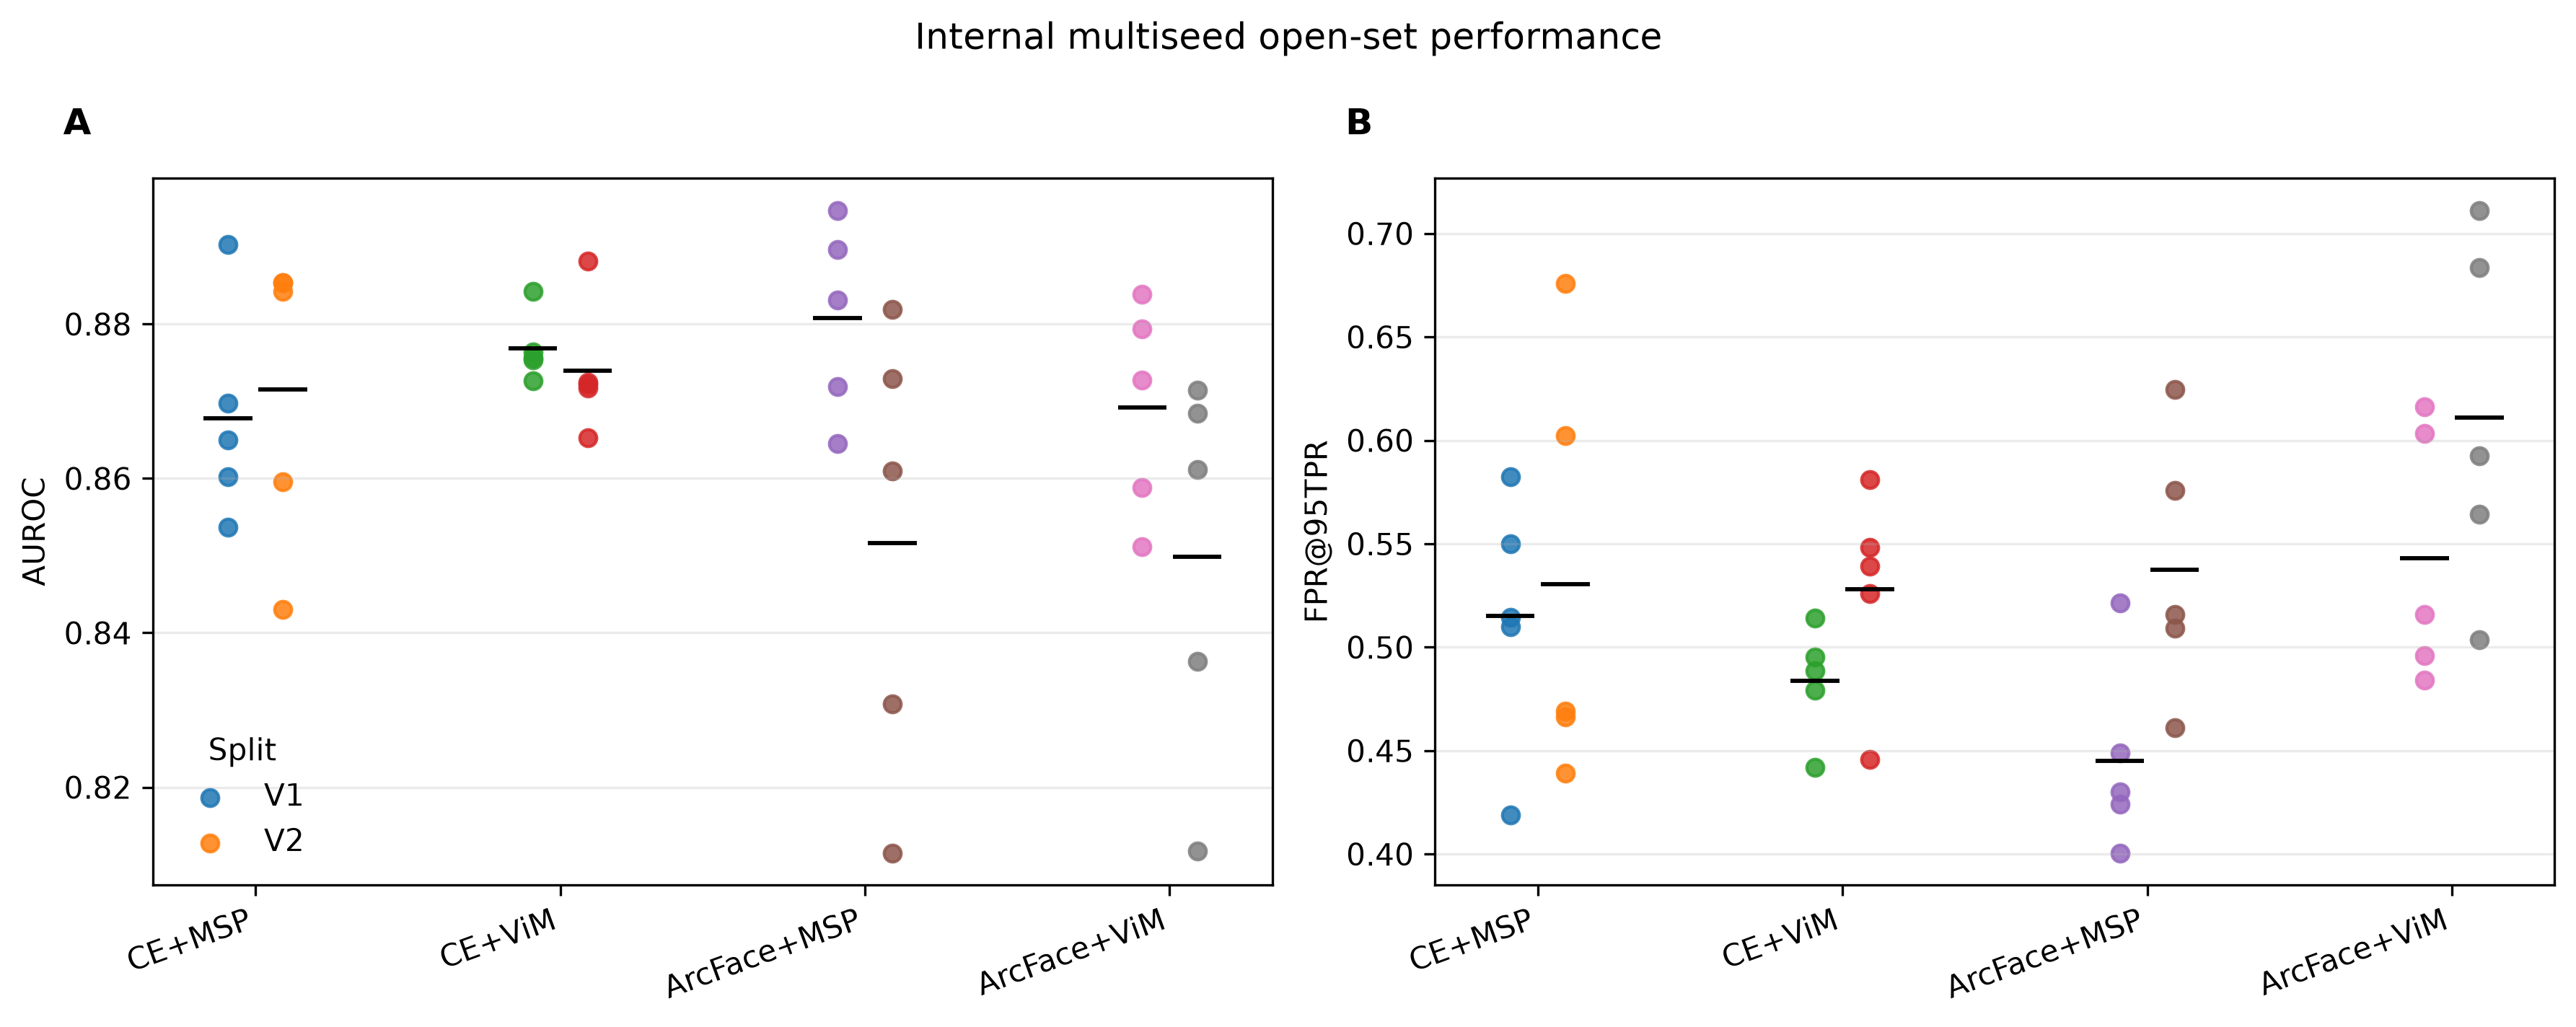
\includegraphics[width=\textwidth]{figure2_internal_performance.png}
\caption{Rendimiento interno de conjunto abierto en MLL23 a través de cinco semillas. Los puntos muestran corridas individuales y los resúmenes horizontales muestran medias a nivel de semilla. El macro-F1 de conjunto cerrado permanece alto, mientras AUROC de conjunto abierto y FPR@95TPR muestran brechas mayores de fiabilidad.}
\label{fig:internal-performance}
\end{figure}

\subsection{Estabilidad del Aprendizaje de Representaciones entre Semillas y Particiones}

ArcFace mejoró algunos resúmenes geométricos de clases conocidas, pero no se reprodujo como una representación superior robusta de conjunto abierto. En V1 con MSP, ArcFace alcanzó AUROC 0.881 $\pm$ 0.012, frente a 0.868 $\pm$ 0.014 para CE+MSP. El delta medio emparejado ArcFace-menos-CE en AUROC fue +0.013, con cuatro de cinco pares de semillas favorables. Sin embargo, el intervalo congelado para este delta pareado incluyó cero. El resultado V2 invirtió la dirección: ArcFace+MSP alcanzó AUROC 0.852 $\pm$ 0.030, mientras CE+MSP alcanzó 0.872 $\pm$ 0.019. El delta V2 emparejado fue -0.020, con solo una de cinco semillas favorable.

El efecto geométrico de ArcFace fue real. La razón de Fisher fue mayor para ArcFace que para CE tanto en V1 como en V2: 3.210 $\pm$ 0.181 frente a 2.703 $\pm$ 0.065 en V1, y 3.234 $\pm$ 0.323 frente a 2.691 $\pm$ 0.092 en V2. La dispersión intraclase fue mucho menor bajo la representación angular normalizada. Sin embargo, los resúmenes geométricos se asociaron débilmente con MSP AUROC a través de las 20 corridas internas: la razón de Fisher tuvo Pearson $r=-0.138$ y Spearman $\rho=0.030$. El resultado separa geometría de clases conocidas de rechazo de desconocidos: mejorar una no garantizó mejorar el otro.

\begin{figure}[htbp]
\centering
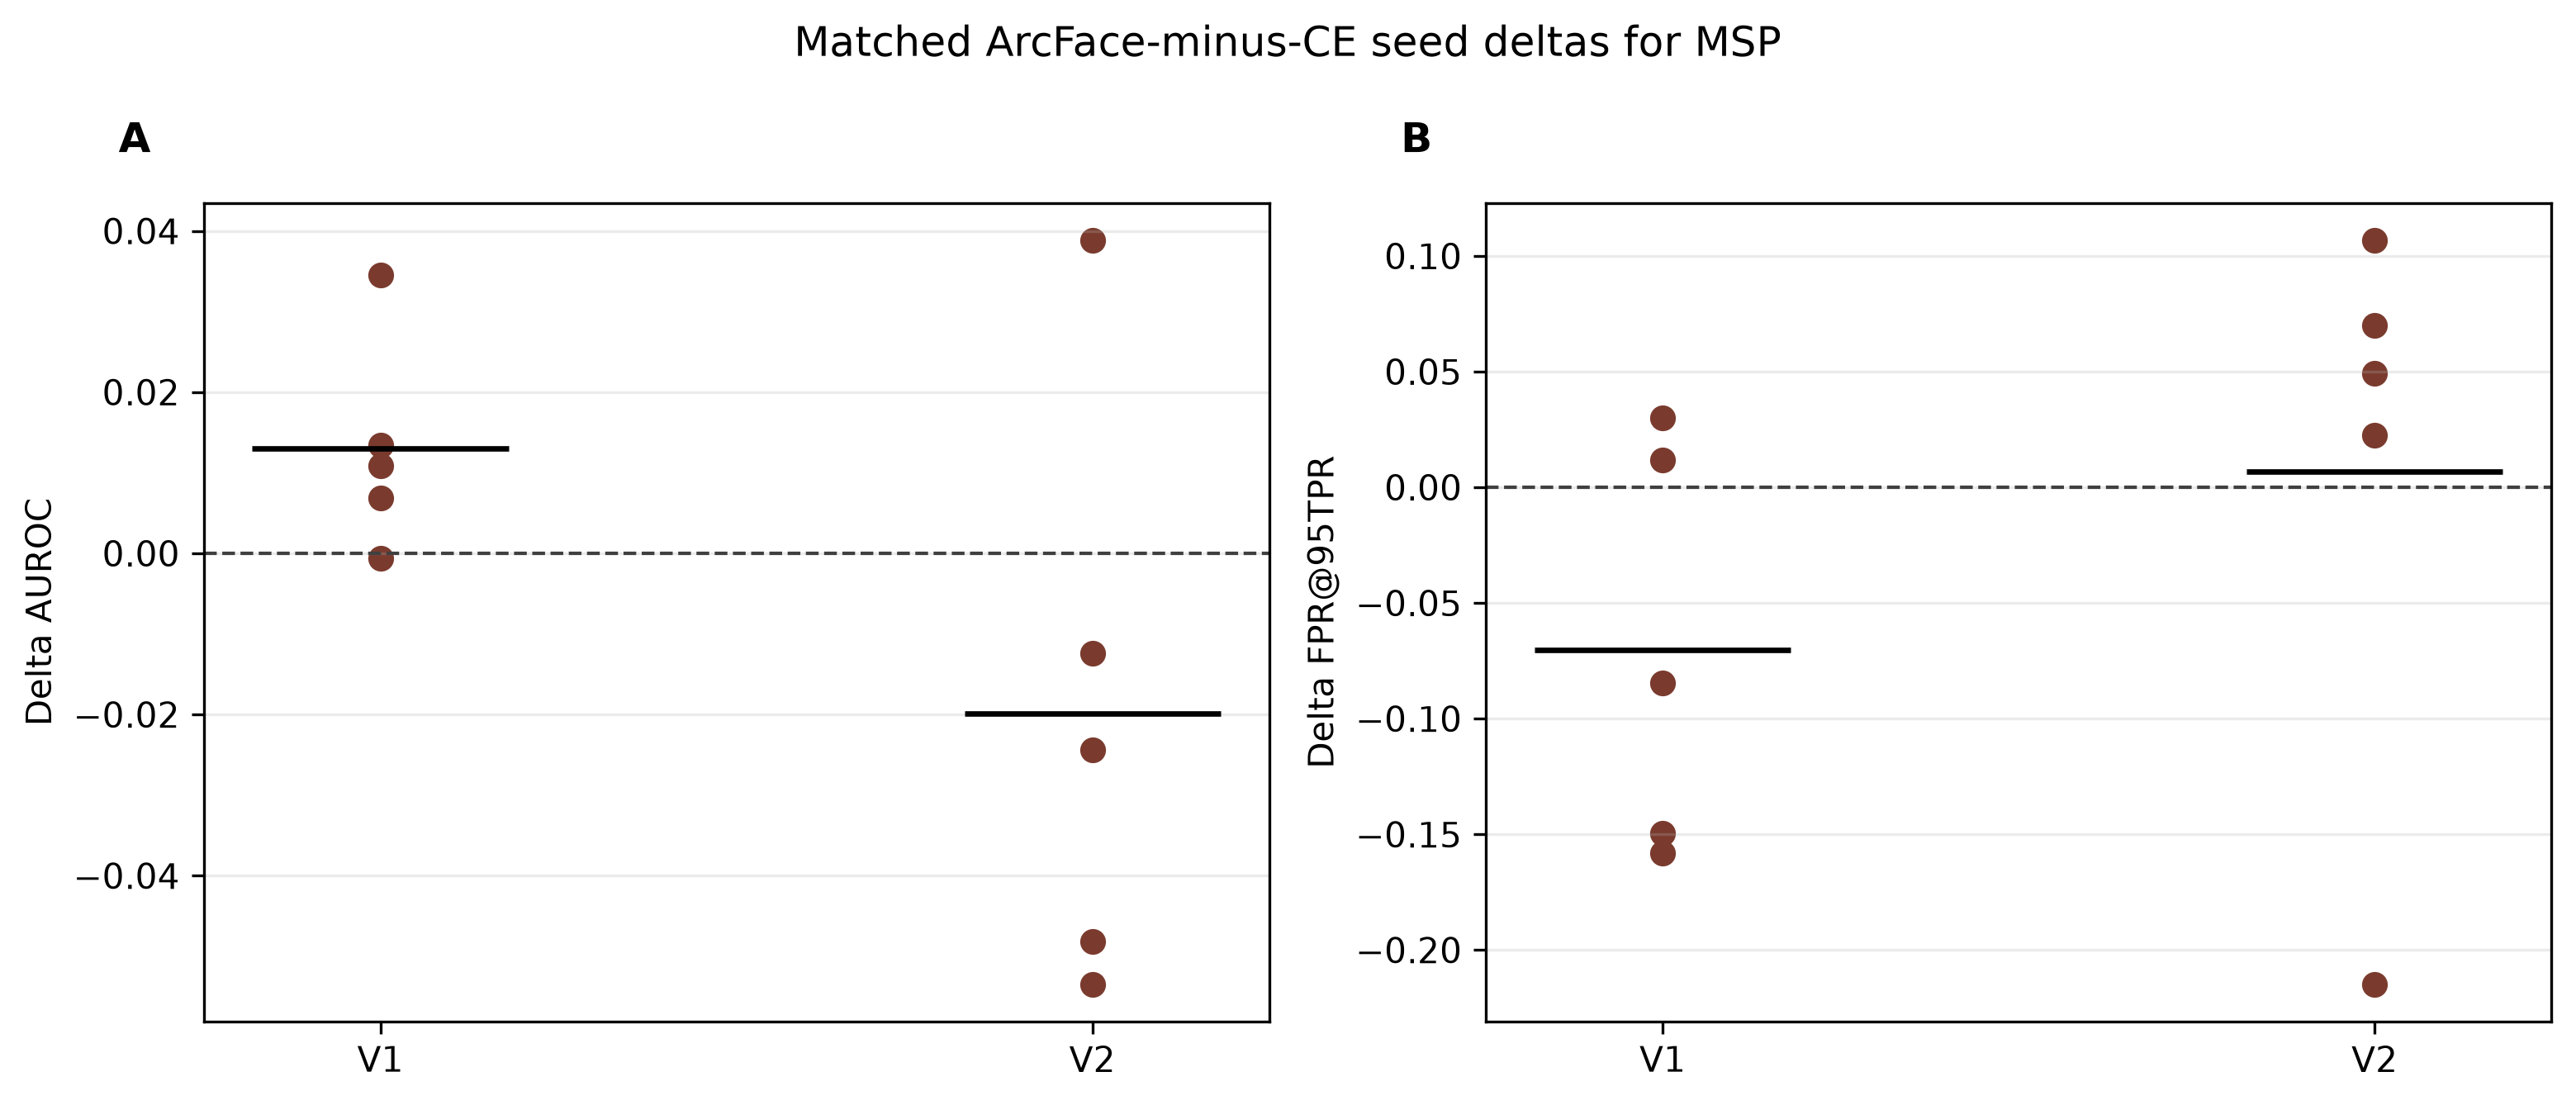
\includegraphics[width=0.92\textwidth]{figure3_arcface_stability.png}
\caption{Deltas emparejados por semilla ArcFace-menos-CE para MSP. Deltas positivos de AUROC favorecen ArcFace; deltas negativos de FPR@95TPR favorecen ArcFace. La tendencia V1 no se reproduce bajo V2, por lo que ArcFace se interpreta como una ablación informativa, no como un método superior confirmado.}
\label{fig:arcface-stability}
\end{figure}

\subsection{Rechazo de Desconocidos Dependiente de Morfología}

La dificultad de rechazo de desconocidos varió fuertemente por morfología. En el análisis externo de morfología CE+ViM, los desconocidos más fáciles por AUROC medio fueron promyelocyte (0.897), myelocyte (0.880), metamyelocyte (0.867), promyelocyte-bilobled (0.856) y erythroblast (0.792). Los más difíciles fueron neutrophil-band (0.526), monoblast (0.575), myeloblast (0.592), lymphocyte-atypical (0.597) y smudge-cell (0.782). Estos valores deben leerse como mediciones del espacio de reconocimiento, no como rankings biológicos de relevancia de enfermedad.

Las morfologías difíciles se alinearon con atractores dominantes de clases conocidas. Las muestras neutrophil-band se asignaron con mayor frecuencia a neutrophil\_segmented. Las muestras monoblast se asignaron con mayor frecuencia a monocyte. Las muestras myeloblast, lymphocyte-atypical y smudge-cell se asignaron frecuentemente a lymphocyte. Este patrón explica por qué AUROC agregado puede ocultar los errores más importantes: algunas morfologías desconocidas no son valores atípicos genéricos, sino vecinas cercanas de la taxonomía conocida.

\begin{figure}[htbp]
\centering
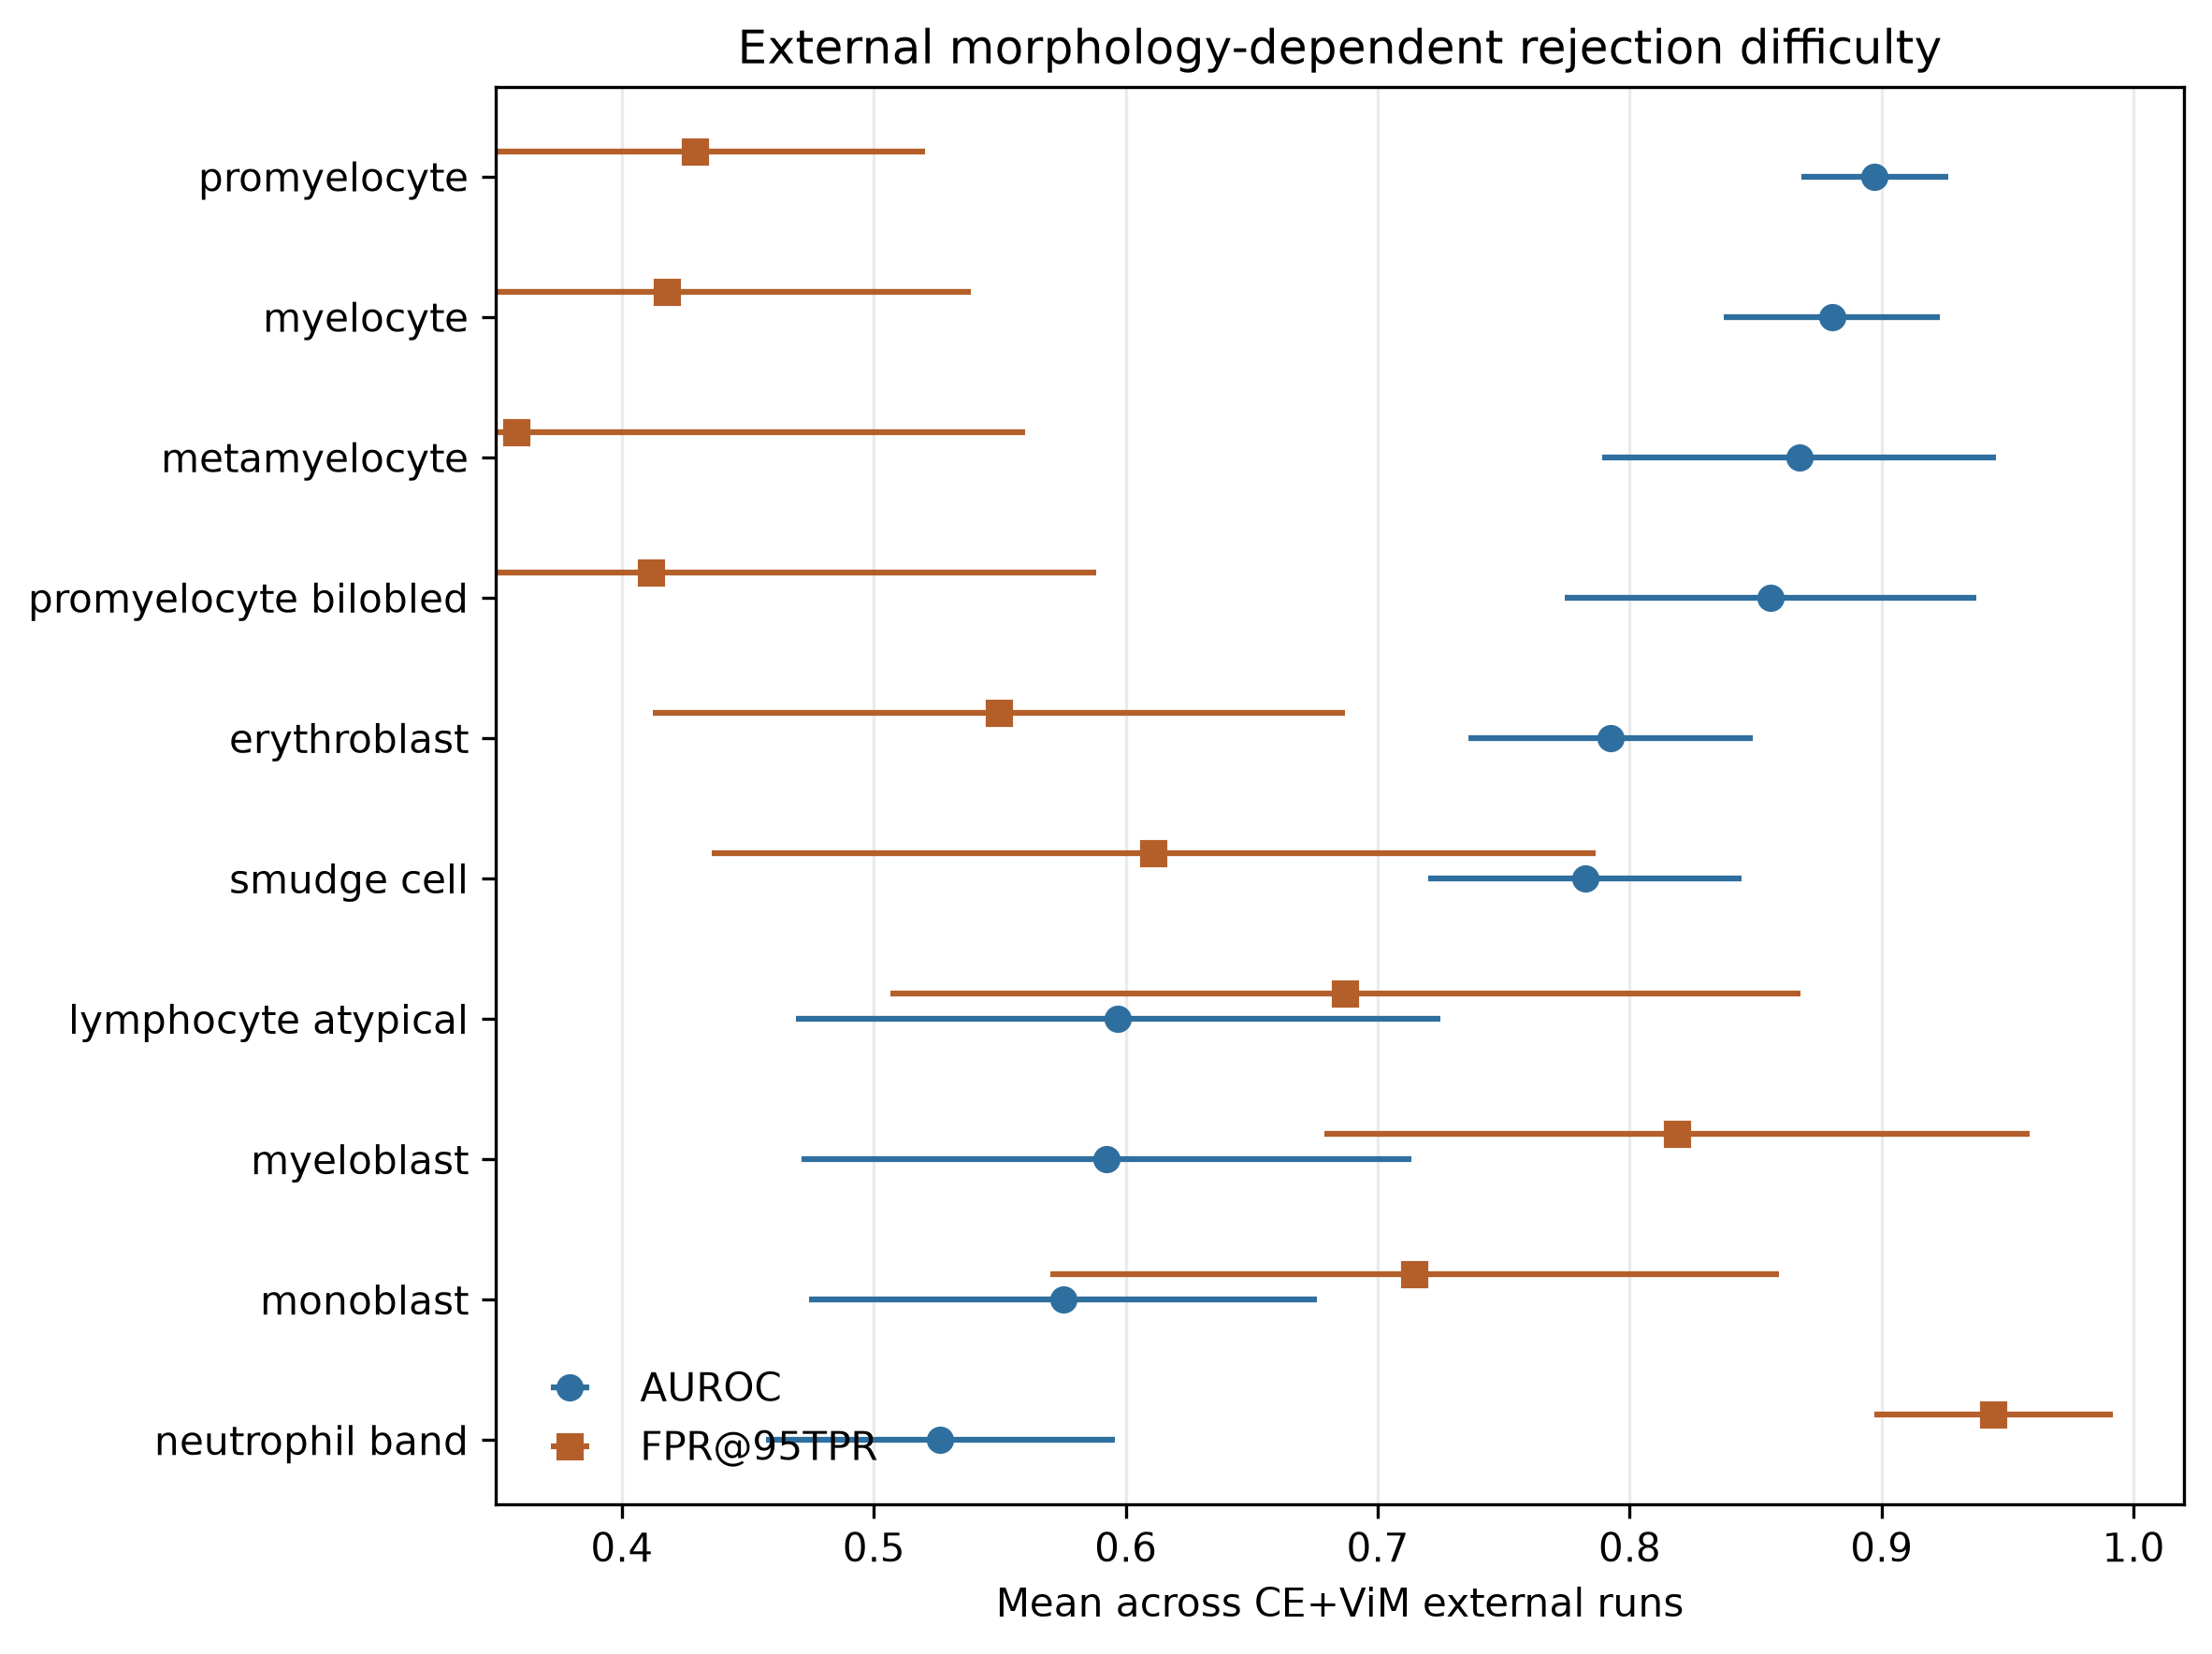
\includegraphics[width=0.86\textwidth]{figure5_external_morphology.png}
\caption{Detección externa de desconocidos dependiente de morfología para CE+ViM. Las barras de error muestran desviación estándar a través de corridas externas congeladas CE+ViM. AUROC bajo para neutrophil-band, monoblast, myeloblast y atypical lymphocyte muestra que el rechazo de desconocidos depende fuertemente de la morfología.}
\label{fig:external-morphology}
\end{figure}

\begin{figure}[htbp]
\centering
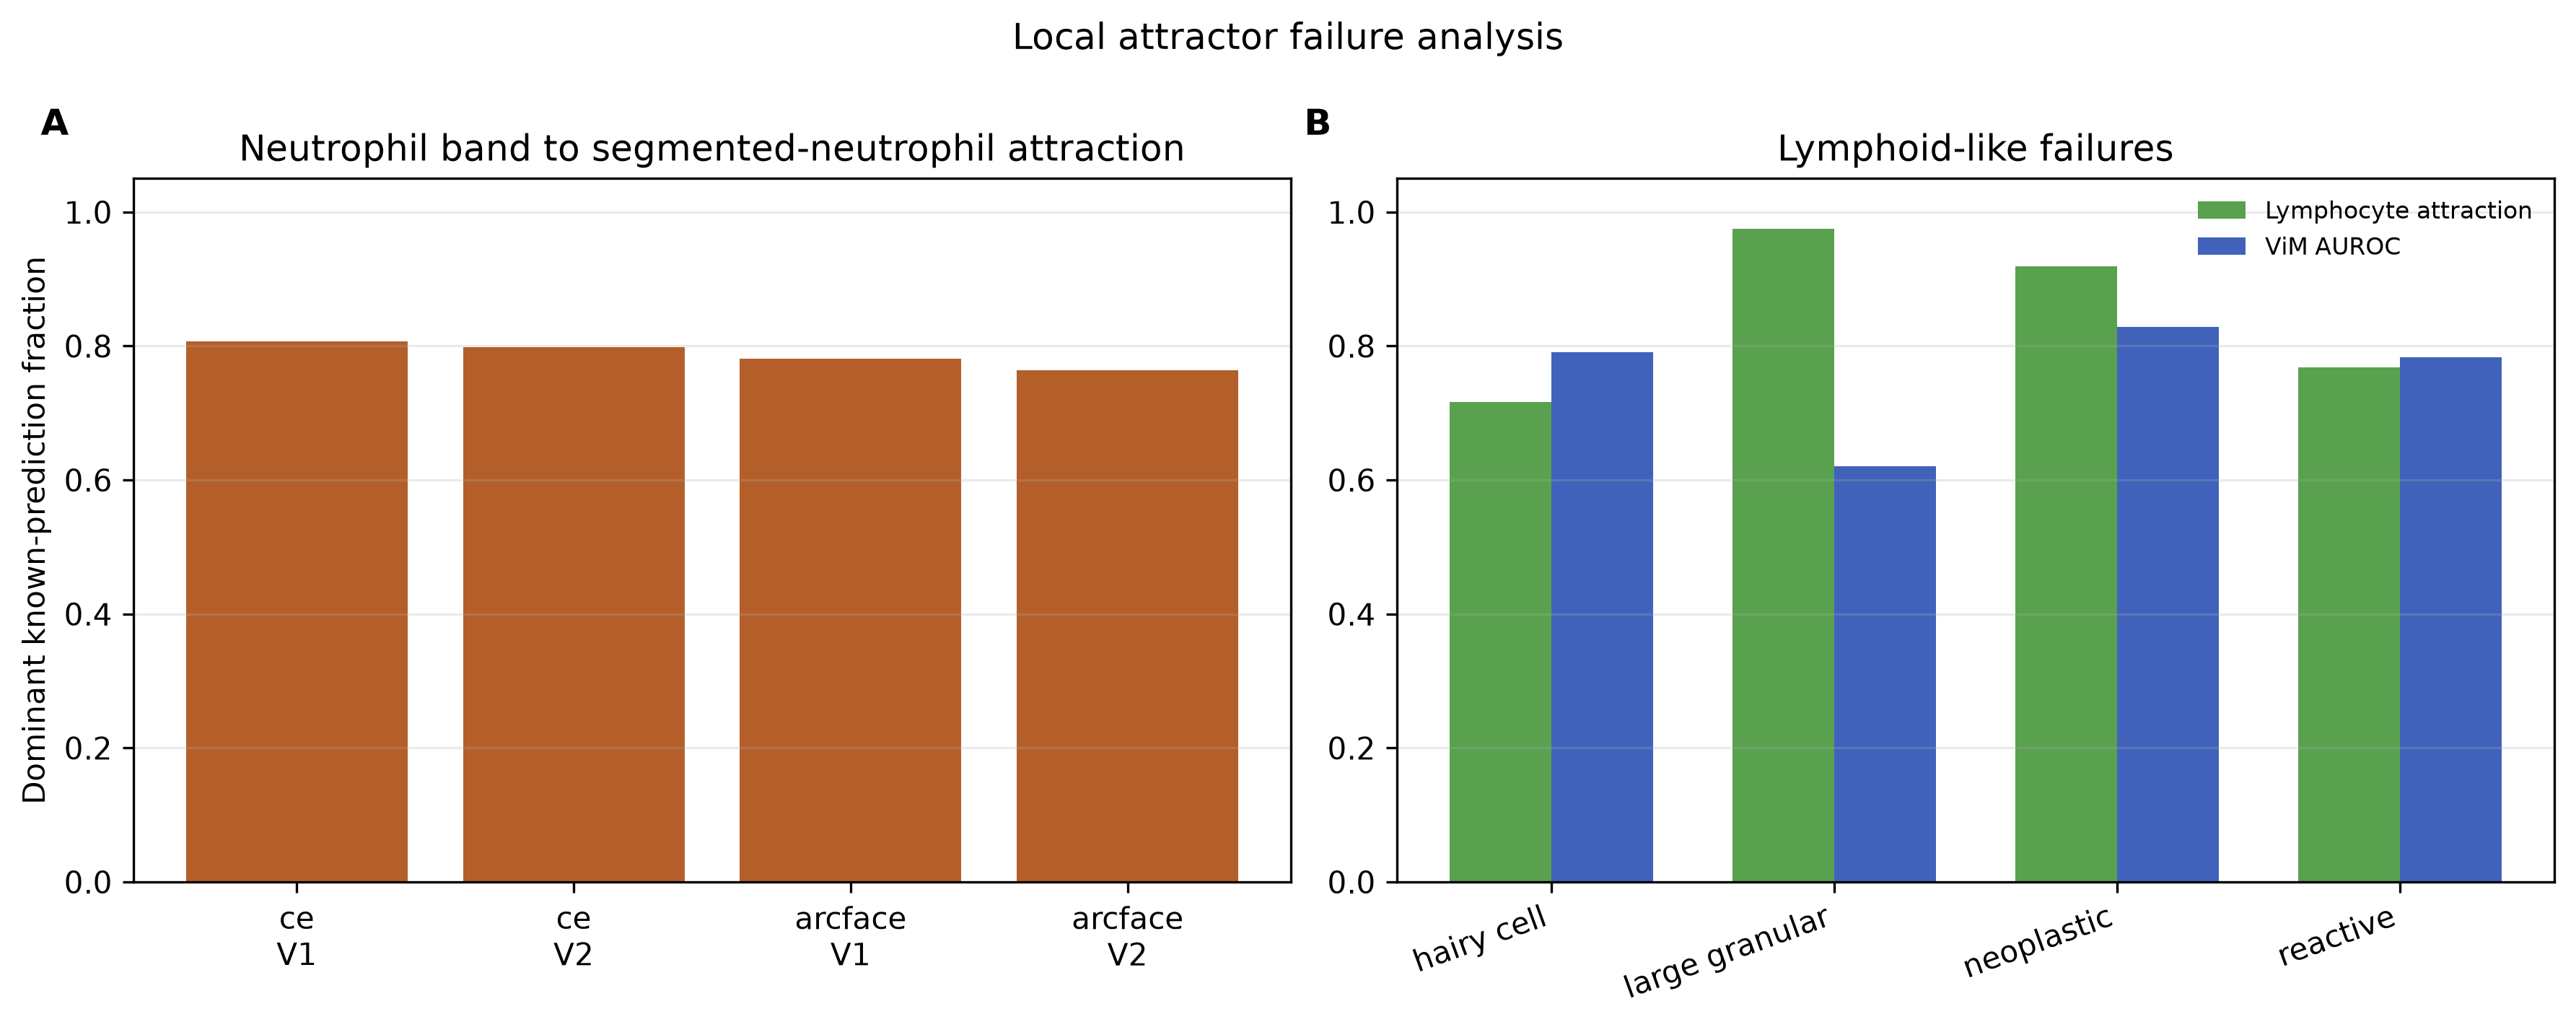
\includegraphics[width=\textwidth]{figure6_failure_cases.png}
\caption{Análisis de atractores de clases conocidas para morfologías desconocidas difíciles representativas. Neutrophil-band es atraída hacia neutrophil\_segmented, monoblast hacia monocyte, y varios desconocidos linfoides hacia lymphocyte.}
\label{fig:failure-cases}
\end{figure}

\subsection{Validación Externa bajo Cambio de Dominio}

El rendimiento externo de conjunto cerrado se degradó sustancialmente en AML-LMU. ArcFace V1 tuvo macro-F1 externo de conjunto cerrado 0.755 $\pm$ 0.009, mientras CE V1 alcanzó 0.711 $\pm$ 0.051. ArcFace V2 alcanzó 0.708 $\pm$ 0.036 y CE V2 alcanzó 0.705 $\pm$ 0.030. Estos resultados estuvieron muy por debajo del macro-F1 interno cercano a 0.97, aunque la exactitud externa de conjunto cerrado permaneció superficialmente alta porque las clases conocidas mapeadas estaban desbalanceadas.

El reconocimiento externo de conjunto abierto fue más débil que el reconocimiento interno para todos los sistemas principales. CE+MSP V1 alcanzó AUROC 0.696 $\pm$ 0.074 y FPR@95TPR 0.796 $\pm$ 0.134. CE+ViM V1 alcanzó AUROC 0.641 $\pm$ 0.090 y FPR@95TPR 0.785 $\pm$ 0.116. ArcFace+MSP V1 alcanzó AUROC 0.690 $\pm$ 0.045 y FPR@95TPR 0.689 $\pm$ 0.107, mientras ArcFace+ViM V1 alcanzó AUROC 0.563 $\pm$ 0.084 y FPR@95TPR 0.879 $\pm$ 0.083.

El patrón externo V2 fue similarmente limitado. CE+MSP V2 alcanzó AUROC 0.630 $\pm$ 0.094 y FPR@95TPR 0.887 $\pm$ 0.100. CE+ViM V2 alcanzó AUROC 0.573 $\pm$ 0.123 y FPR@95TPR 0.867 $\pm$ 0.138. ArcFace+MSP V2 alcanzó AUROC 0.696 $\pm$ 0.069 y FPR@95TPR 0.723 $\pm$ 0.162. ArcFace+ViM V2 alcanzó AUROC 0.632 $\pm$ 0.087 y FPR@95TPR 0.851 $\pm$ 0.062.

\begin{table}[htbp]
\centering
\small
\resizebox{\textwidth}{!}{%
\begin{tabular}{l c c c c c}
\toprule
Sistema & Partición de entrenamiento & AUROC & FPR@95TPR & OSCR & Macro-F1 cerrado \\
\midrule
CE+MSP & V1 & 0.696 $\pm$ 0.074 & 0.796 $\pm$ 0.134 & 0.664 $\pm$ 0.068 & 0.711 $\pm$ 0.051 \\
CE+MSP & V2 & 0.630 $\pm$ 0.094 & 0.887 $\pm$ 0.100 & 0.599 $\pm$ 0.081 & 0.705 $\pm$ 0.030 \\
CE+ViM & V1 & 0.641 $\pm$ 0.090 & 0.785 $\pm$ 0.116 & 0.608 $\pm$ 0.078 & 0.711 $\pm$ 0.051 \\
CE+ViM & V2 & 0.573 $\pm$ 0.123 & 0.867 $\pm$ 0.138 & 0.540 $\pm$ 0.107 & 0.705 $\pm$ 0.030 \\
ArcFace+MSP & V1 & 0.690 $\pm$ 0.045 & 0.689 $\pm$ 0.107 & 0.664 $\pm$ 0.043 & 0.755 $\pm$ 0.009 \\
ArcFace+MSP & V2 & 0.696 $\pm$ 0.069 & 0.723 $\pm$ 0.162 & 0.660 $\pm$ 0.075 & 0.708 $\pm$ 0.036 \\
ArcFace+ViM & V1 & 0.563 $\pm$ 0.084 & 0.879 $\pm$ 0.083 & 0.542 $\pm$ 0.080 & 0.755 $\pm$ 0.009 \\
ArcFace+ViM & V2 & 0.632 $\pm$ 0.087 & 0.851 $\pm$ 0.062 & 0.599 $\pm$ 0.086 & 0.708 $\pm$ 0.036 \\
\bottomrule
\end{tabular}
}
\caption{Resultados externos AML-LMU solo de prueba. Los valores son media $\pm$ desviación estándar sobre cinco semillas de entrenamiento. No se usa ningún dato AML-LMU para entrenamiento, adaptación, calibración ni selección metodológica.}
\label{tab:external}
\end{table}

\begin{figure}[htbp]
\centering
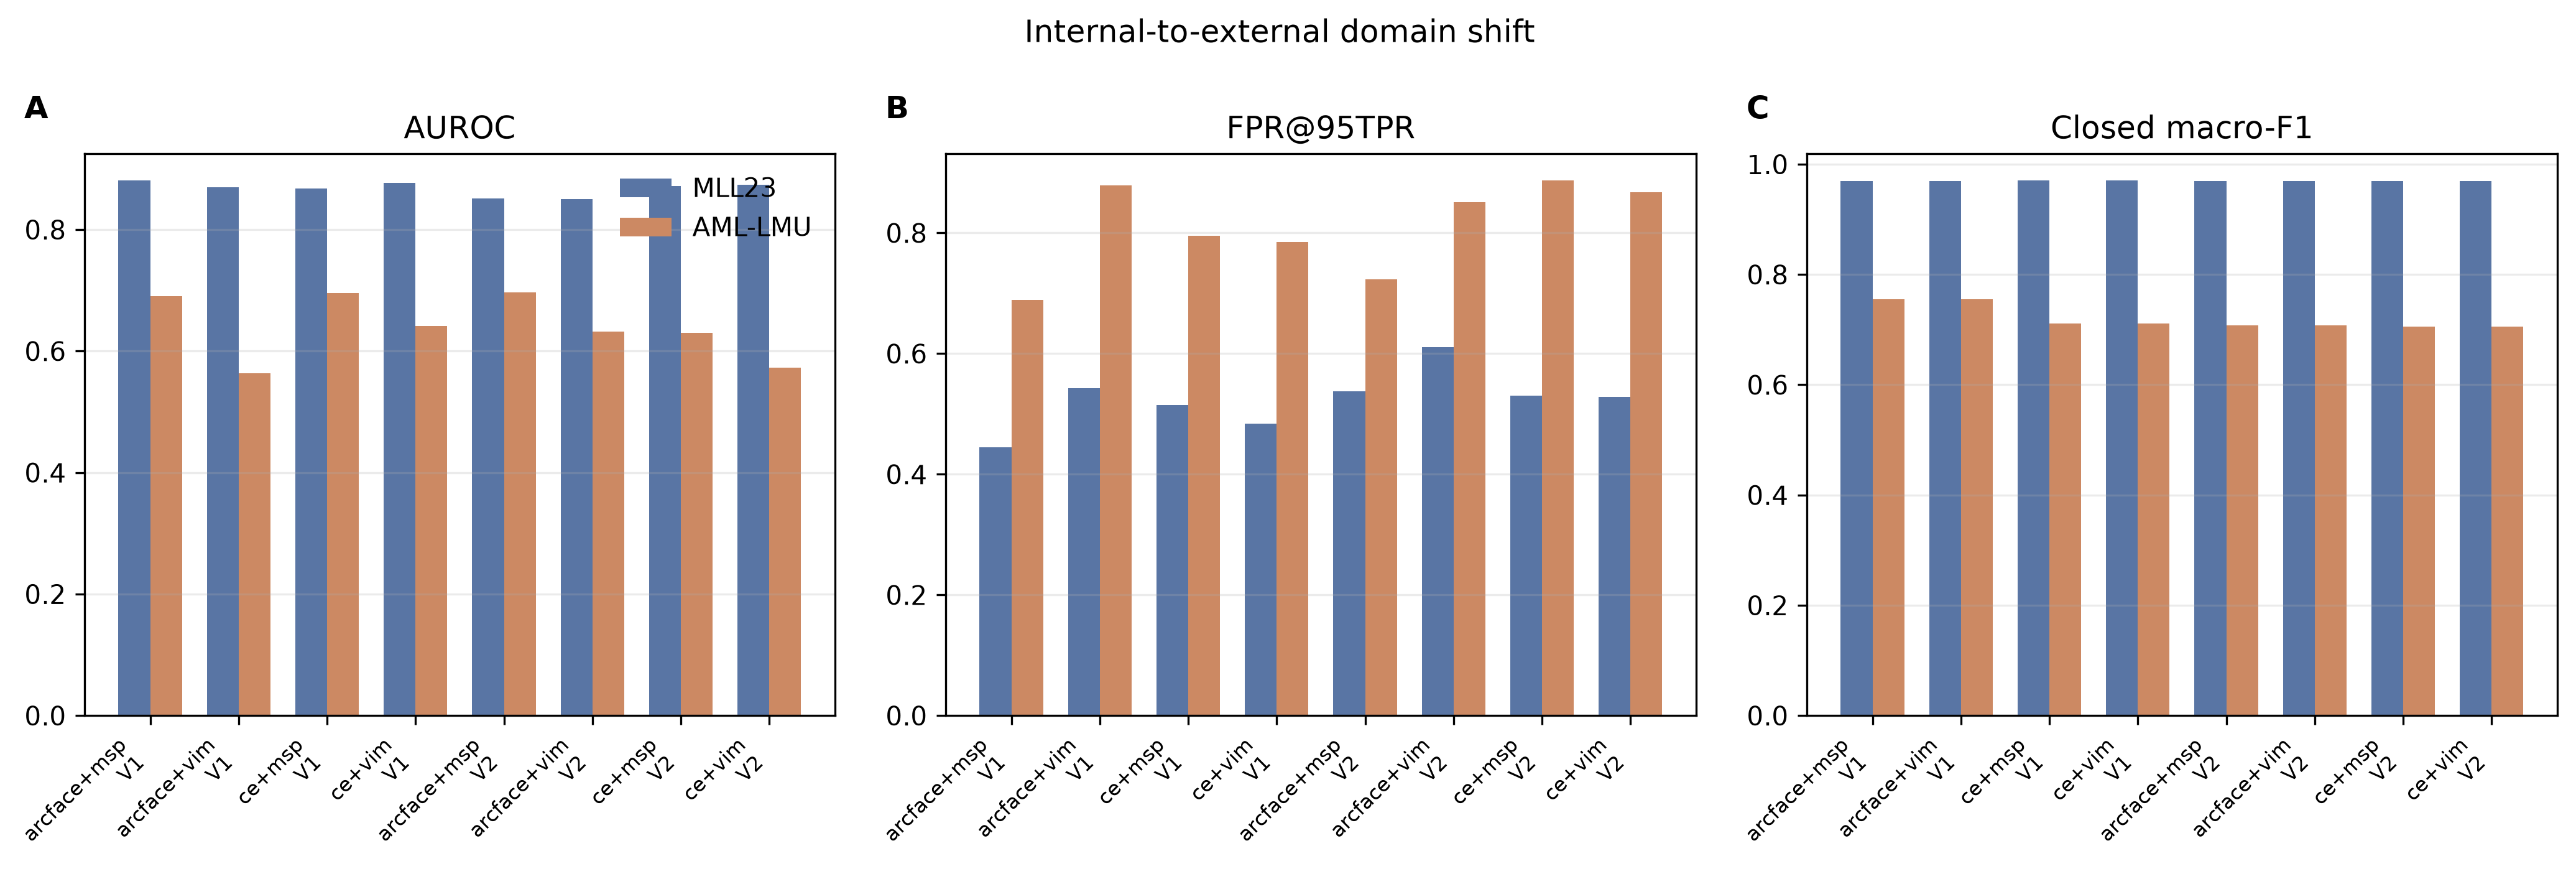
\includegraphics[width=\textwidth]{figure4_domain_shift.png}
\caption{Cambio de dominio interno-a-externo para los sistemas principales. AML-LMU es un dominio solo de prueba: no se realiza entrenamiento externo, calibración de umbrales, selección metodológica, ajuste PCA, ajuste ViM ni selección de preprocesamiento.}
\label{fig:domain-shift}
\end{figure}

\subsection{Inestabilidad de Ranking Interno-a-Externo}

Los rankings metodológicos internos no se transfirieron limpiamente. CE+ViM fue el basal conservador de estabilidad interna, pero MSP superó a ViM por AUROC externo medio tanto para CE como para ArcFace en V1 y V2. Por ejemplo, CE+MSP V1 alcanzó AUROC externo 0.696 frente a 0.641 para CE+ViM V1. CE+MSP V2 alcanzó 0.630 frente a 0.573 para CE+ViM V2. ArcFace mostró una ventaja externa similar para MSP. El basal externo práctico es por tanto CE+MSP, mientras CE+ViM permanece como comparador internamente estable. El manuscrito no promueve un ganador universal único.

La magnitud del cambio de dominio fue grande. Para CE+ViM, AUROC cayó de 0.877 a 0.641 en V1 y de 0.874 a 0.573 en V2. FPR@95TPR aumentó de 0.484 a 0.785 en V1 y de 0.528 a 0.867 en V2. Macro-F1 cerrado cayó 0.260 en V1 y 0.264 en V2. Estos cambios pareados apoyan la conclusión central de validez externa: las diferencias de adquisición y dominio taxonómico cambiaron materialmente tanto el comportamiento de conjunto cerrado como el de conjunto abierto.

\subsection{Análisis Secundario de Topología y Geometría}

La homología persistente cubical no aportó beneficio predictivo robusto de conjunto abierto bajo el protocolo evaluado. Las características TDA-only codificaron alguna información de clase, con macro-F1 cerrado TDA-only congelado que alcanzó aproximadamente 0.828, pero AUROC de conjunto abierto permaneció aproximadamente 0.55--0.58 para variantes TDA-only. La fusión Deep+TDA degradó el basal profundo principal en lugar de mejorarlo. Este resultado es una ablación negativa, no una afirmación de que la morfología celular carezca de estructura topológica.

La topología Vietoris-Rips fue más útil como análisis descriptivo de embeddings aprendidos. El análisis congelado incluyó 500 análisis de nubes de puntos y 1,000 filas de resumen $H_0$/$H_1$ a través de dominios internos y externos, dos particiones, dos representaciones, cinco semillas, clases conocidas y morfologías desconocidas difíciles seleccionadas. Las relaciones topología-OSR fueron débiles e inconsistentes. Para MSP AUROC, la persistencia máxima media $H_1$ conocida tuvo Pearson $r=0.148$ y Spearman $\rho=0.014$, mientras la razón de Fisher tuvo Pearson $r=-0.138$ y Spearman $\rho=0.030$. Estos resultados no apoyan una afirmación topológica predictiva ni causal.

\begin{figure}[htbp]
\centering
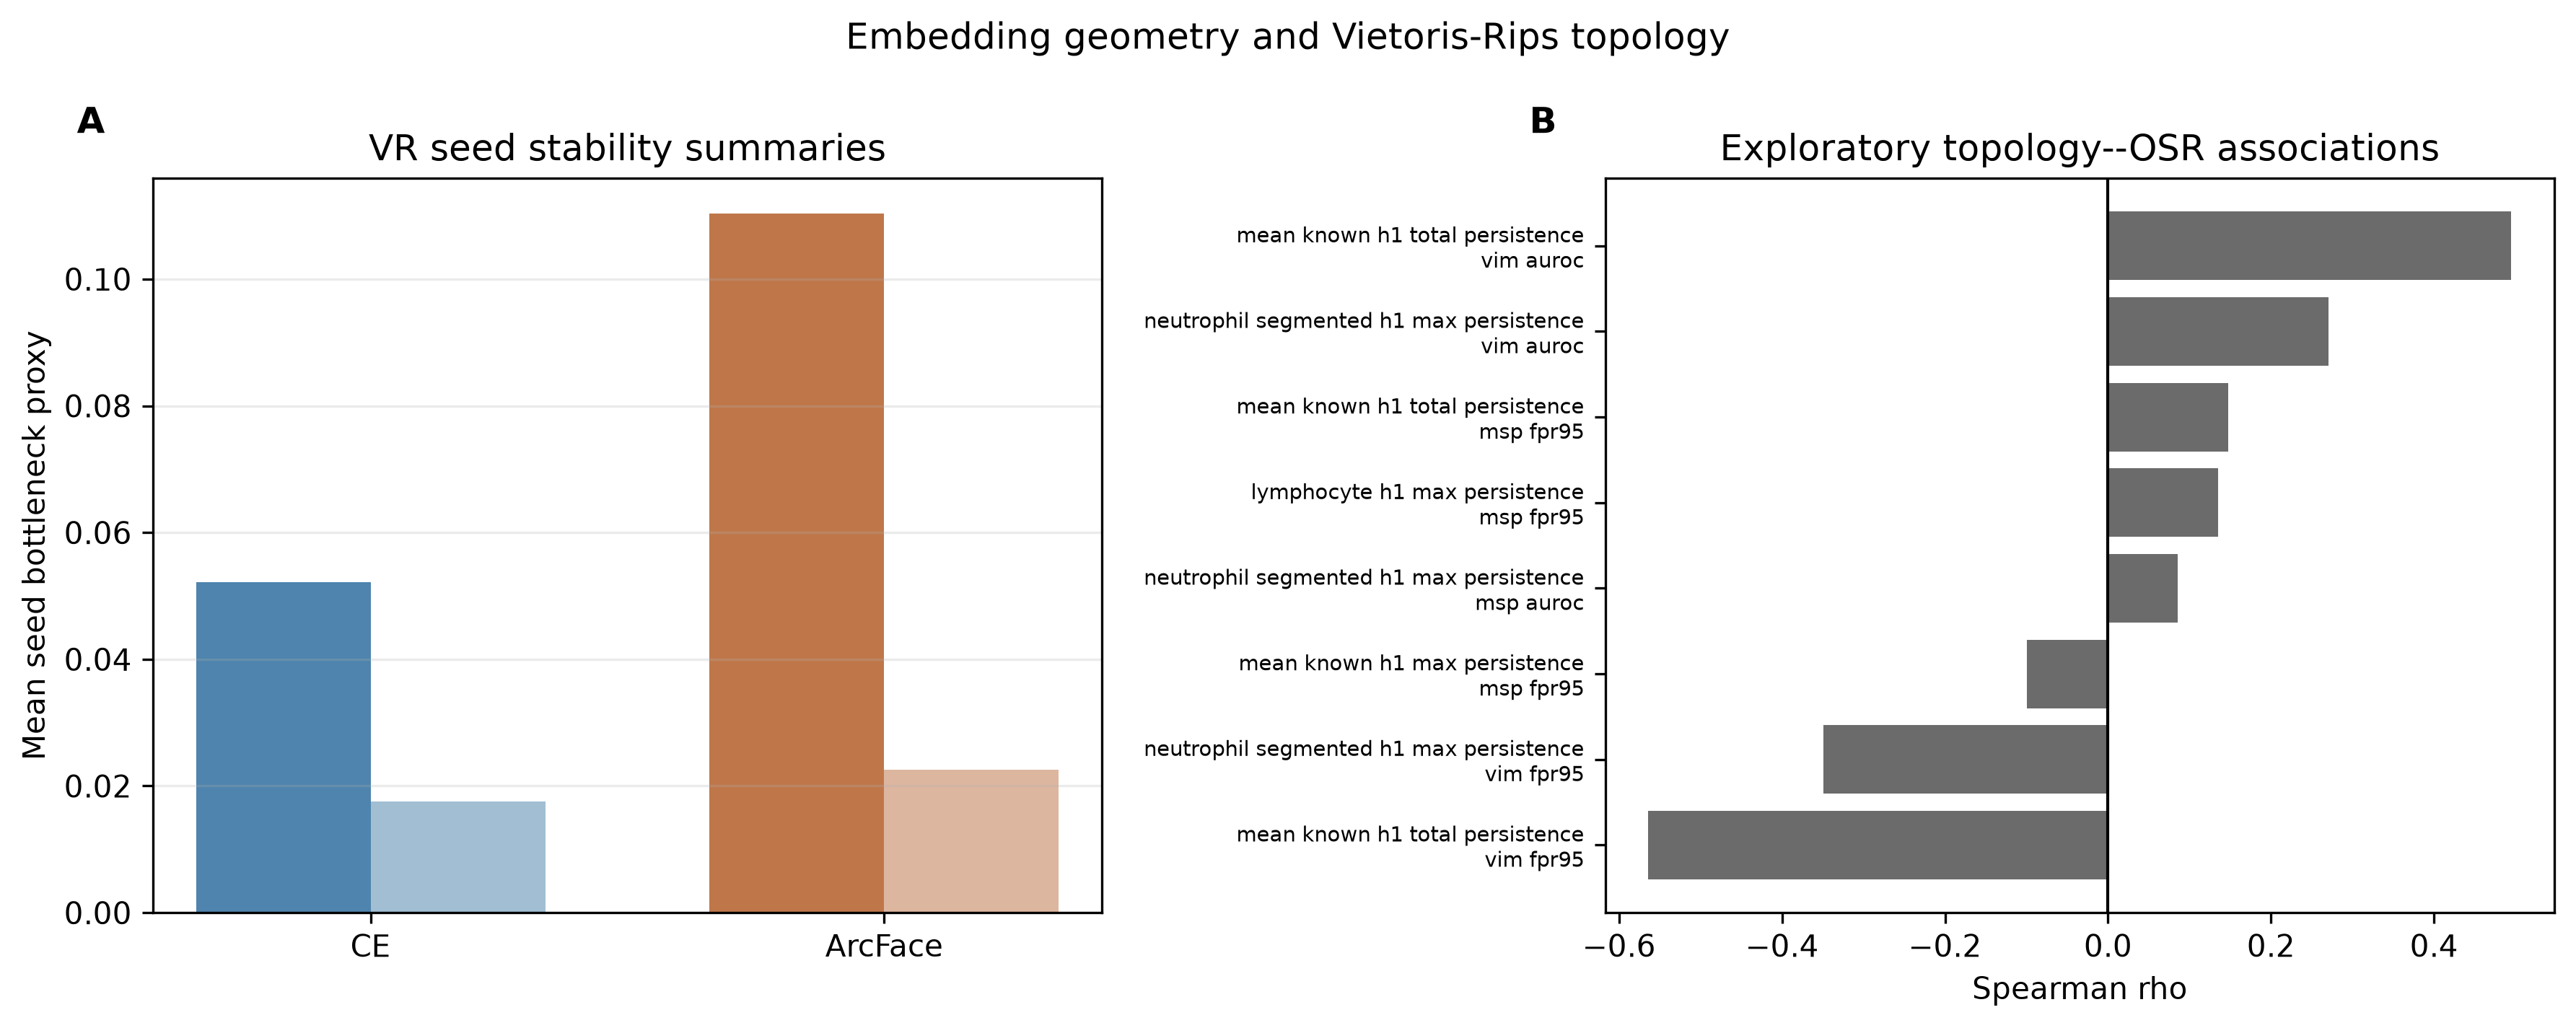
\includegraphics[width=\textwidth]{figure7_topology.png}
\caption{Resúmenes secundarios de topología Vietoris-Rips y asociaciones exploratorias con métricas OSR. El análisis describe la geometría de embeddings después de congelar los resultados predictivos y no se usa para selección de modelos, umbralización ni predicción.}
\label{fig:topology}
\end{figure}

\section{Discusión}

\subsection{El Rendimiento de Conjunto Cerrado Es Evidencia Insuficiente de Fiabilidad de Conjunto Abierto}

El resultado primario es la coexistencia de clasificación leucocitaria fuerte de conjunto cerrado y fiabilidad incompleta de conjunto abierto. Internamente, tanto CE como ArcFace ResNet18 alcanzaron macro-F1 cercano a 0.97 en leucocitos maduros conocidos. Si la evaluación terminara ahí, los sistemas parecerían altamente fiables. Las métricas de conjunto abierto cambiaron la interpretación. CE+ViM alcanzó AUROC interno alrededor de 0.87, pero FPR@95TPR permaneció cerca de 0.48--0.53. Luego, AUROC externo cayó aproximadamente a 0.57--0.70 en los sistemas principales, con FPR@95TPR alto. Estos hallazgos muestran que la capacidad de clasificar leucocitos conocidos no implica capacidad para rechazar morfologías no vistas.

Esto no es una contradicción. Las métricas de conjunto cerrado condicionan la suposición de que la etiqueta correcta está en el conjunto de etiquetas del modelo. El reconocimiento de conjunto abierto prueba un comportamiento diferente: si una entrada debe ser retenida fuera de la taxonomía conocida. Un modelo puede tomar decisiones exactas para clases conocidas y aun así asignar una muestra desconocida morfológicamente relacionada a la clase conocida más cercana con alta confianza. Para morfología hematológica, se espera que ese comportamiento sea común porque las clases no vistas a menudo están biológica y visualmente relacionadas con clases conocidas, no son corrupciones arbitrarias de imagen.

\subsection{La Similitud Morfológica Produce Fallo Estructurado}

El análisis de fallos indica que los errores desconocidos están estructurados por morfología. Neutrophil-band fue difícil externamente y fue atraída dominantemente hacia neutrophil\_segmented. Monoblast fue atraída dominantemente hacia monocyte. Myeloblast, atypical lymphocyte y smudge-cell mostraron atracción hacia lymphocyte en el análisis externo CE+ViM. No son errores aleatorios. Reflejan vecindarios del espacio de reconocimiento plausibles bajo morfología visual, aunque el protocolo requiere que estas muestras permanezcan fuera de la taxonomía conocida.

Esta observación tiene dos implicaciones. Primero, AUROC agregado es necesario pero insuficiente. Un sistema con rendimiento medio aceptable aún puede fallar en las categorías desconocidas más interesantes clínica o morfológicamente. Segundo, las evaluaciones hematológicas de conjunto abierto deben reportar comportamiento por morfología, incluidos atractores de clases conocidas e incertidumbre en clases pequeñas. El presente estudio no afirma que estos atractores prueben causalidad biológica. Afirma que los errores de conjunto abierto dependen de la morfología y, por tanto, requieren análisis a nivel de morfología.

\subsection{Una Mejor Geometría de Clases Conocidas No Garantiza Mejor Separación de Desconocidos}

ArcFace es informativo precisamente porque mejoró algunos resúmenes geométricos de clases conocidas sin producir una ventaja robusta de conjunto abierto. La mayor razón de Fisher y la menor dispersión intraclase muestran que la representación cambió en la dirección prevista para clases conocidas. Sin embargo, la ventaja AUROC MSP de V1 no se confirmó en V2, y la evidencia emparejada por semilla no apoyó una afirmación global de superioridad. Externamente, ArcFace+MSP fue competitivo en algunas comparaciones, especialmente V2, pero esto no borra el fallo de confirmación interna.

El resultado advierte contra un atajo común: asumir que clústeres conocidos compactos mejoran automáticamente el rechazo de desconocidos. Las muestras desconocidas se juzgan en relación con la geometría aprendida de clases conocidas. Si una morfología no vista cae cerca de una clase conocida, una representación más compacta o angular aún puede tratarla como un miembro confiado de ese vecindario conocido. La evidencia apoya por tanto una interpretación conservadora: ArcFace es una ablación útil de representación y una fuente de información, no un método confirmado para reconocimiento robusto de leucocitos en conjunto abierto.

\subsection{El Cambio de Dominio Externo Cambia el Problema}

AML-LMU es la prueba de estrés decisiva del artículo. Difiere de MLL23 en fuente, contexto de adquisición, dimensiones de imagen, composición de clases y taxonomía fuente. El protocolo solo de prueba evita que la adaptación externa oculte la pregunta de generalización. Bajo este diseño, todos los sistemas principales se degradaron. Macro-F1 cerrado cayó aproximadamente 0.21--0.26 según representación y partición, y AUROC de conjunto abierto cayó para todos los sistemas. El ranking metodológico también cambió: ViM fue estable internamente, pero MSP fue más fuerte externamente en las comparaciones principales CE y ArcFace.

Esta inestabilidad de ranking importa para la práctica investigadora. Si se selecciona un método solo porque rinde mejor internamente, la selección puede no transferirse a un nuevo dominio de adquisición. A la inversa, si un método parece fuerte externamente tras muchas elecciones de ajuste externo, quizá ya no sea una prueba limpia de generalización. El presente estudio elige la ruta más estricta: los datos externos permanecen intactos hasta la evaluación final. El rendimiento resultante no es halagador, pero es científicamente útil porque mide un modo de fallo realista.

\subsection{Qué Revela y Qué No Revela la Homología Persistente}

La homología persistente tiene un papel disciplinado pero secundario. La homología persistente cubical se probó como familia de características predictivas y no aportó utilidad complementaria robusta para detección de desconocidos. El resultado negativo debe permanecer en el artículo porque evita que el título y el encuadre sugieran un método topológico no respaldado. También documenta que la topología derivada de imagen, tal como se implementó en los experimentos congelados, no resolvió el problema de conjunto abierto.

La homología persistente Vietoris-Rips es diferente. Describe la topología de nubes de embeddings aprendidos después de fijar los experimentos predictivos. La variación observada por semilla, partición y dominio puede ayudar a caracterizar el comportamiento de representación, pero las correlaciones topología-OSR son débiles e inconsistentes. Por tanto, el estudio evita afirmaciones causales. La topología puede ser útil para diagnósticos exploratorios futuros, pero la evidencia presente no apoya usarla como predictor de fiabilidad de conjunto abierto.

\subsection{Implicaciones para la Evaluación}

Los resultados apoyan una lista conservadora de evaluación para sistemas de morfología hematológica. Las clases desconocidas deben definirse antes de producir métricas. Las muestras desconocidas deben permanecer solo de prueba. Debe auditarse la fuga exacta y de casi duplicados, y no debe afirmarse validación a nivel de paciente cuando no hay identificadores de paciente. Los resultados deben reportarse entre semillas, externamente cuando sea posible y por morfología desconocida. Las afirmaciones deben distinguir clasificación de clases conocidas, reconocimiento de conjunto abierto y diagnóstico a nivel de paciente.

Por tanto, este manuscrito se posiciona mejor como un estudio empírico riguroso que como un artículo de nueva arquitectura. Su contribución no es que CE, ArcFace, ViM, MSP u homología persistente sean la respuesta final. Su contribución es la evidencia de que un clasificador leucocitario plausible de conjunto cerrado puede fallar de maneras estructuradas cuando la taxonomía está incompleta y cambia el dominio de adquisición.

El estudio también aboga por un estilo distinto de reporte en benchmarks de morfología biomédica. Un único número de exactitud de la misma fuente es fácil de comunicar, pero puede ocultar si el modelo aprendió una representación morfológica robusta o una regla de decisión más estrecha y específica de fuente. Reportar variación por semilla, sensibilidad de partición, transferencia externa y comportamiento de desconocidos por morfología hace la historia menos ordenada, pero refleja mejor la pregunta de fiabilidad que surge cuando los modelos se reutilizan fuera de su inventario original de etiquetas. Esto es particularmente importante en escenarios de conjunto abierto, donde el comportamiento más relevante puede ser la decisión de no asignar una clase conocida.

Finalmente, los resultados clarifican el papel de la evidencia negativa. Los análisis ArcFace y de homología persistente no produjeron una historia simple de mejora, pero previenen conclusiones engañosas. ArcFace muestra que mejor geometría de clases conocidas no equivale a mejor rechazo de desconocidos. La homología persistente cubical muestra que los descriptores evaluados de topología de imagen no rescataron el rendimiento de conjunto abierto. Los resúmenes Vietoris-Rips muestran que la topología de embeddings puede describirse sin promoverse como predictor. Mantener estos hallazgos en el manuscrito hace que la evaluación sea más reproducible y menos vulnerable al reporte selectivo.

\section{Limitaciones}

Varias limitaciones restringen la interpretación de este estudio. Primero, MLL23 es el único conjunto interno y AML-LMU es el único dominio externo. Se necesitarían conjuntos independientes adicionales para estimar el rango de comportamiento bajo cambio de dominio entre escáneres, tinciones, laboratorios, políticas de anotación y poblaciones de pacientes. Segundo, los identificadores confiables de paciente o grupo de adquisición no están disponibles en los manifiestos MLL23 de trabajo. La partición V2 es un análisis conservador de sensibilidad exacta y de casi duplicados, no validación a nivel de paciente. AML-LMU documenta conteos de sujetos en la colección fuente, pero los identificadores de paciente no estuvieron disponibles en los campos auditados usados para este proyecto.

Tercero, las clases desconocidas se definen por el protocolo. Están fuera de la taxonomía conocida de entrenamiento, pero no definen malignidad, leucemia, diagnóstico anormal ni hallazgo clínico positivo. Cuarto, la distribución de clases está desbalanceada tanto en datos internos como externos. Esto motiva macro-F1, exactitud balanceada, resultados por morfología y métricas de conjunto abierto, pero el desbalance todavía afecta la incertidumbre alrededor de clases externas desconocidas pequeñas como atypical lymphocytes, metamyelocytes, monoblasts y smudge cells.

Quinto, la familia de modelos se limita a variantes ResNet18 preentrenadas en ImageNet con configuraciones de entrenamiento congeladas. El estudio usa cinco semillas, lo cual es más fuerte que un reporte de una sola corrida, pero no exhaustivo. Sexto, ArcFace se evalúa con un margen y escala congelados. Un ajuste posterior podría cambiar los resultados, pero ajustar después de ver resultados confirmatorios reabriría la selección metodológica y debilitaría el diseño de evaluación congelada. Séptimo, el conjunto interno desconocido fue inspeccionado durante análisis previos, por lo que los hallazgos explicativos internos no deben tratarse como descubrimiento independiente. Por ello, el análisis externo solo de prueba es especialmente importante.

Octavo, no se realiza adaptación externa. Esto fortalece la afirmación de validación externa, pero no estima el mejor rendimiento posible tras adaptación de dominio, normalización de tinción, calibración externa o fine-tuning en dominio objetivo. Noveno, las conclusiones de homología persistente se limitan a las filtraciones, vectorizadores, diseños de fusión, tamaños de muestra y estadísticas de resumen evaluados. No deben generalizarse a todos los métodos topológicos. Finalmente, el estudio es una evaluación de investigación en conjuntos públicos, no una evaluación prospectiva de flujo clínico, no una tarea diagnóstica a nivel de paciente y no una garantía de que los desconocidos definidos por el conjunto cubran toda la diversidad de la morfología hematológica real.

\section{Conclusión}

Este estudio evalúa el reconocimiento de conjunto abierto de morfologías leucocitarias no vistas bajo una taxonomía congelada y cambio de dominio externo. La conclusión principal es que un alto rendimiento de conjunto cerrado no basta: los modelos ResNet18 alcanzaron macro-F1 interno de clases conocidas cercano a 0.97, pero el rechazo de desconocidos permaneció imperfecto, dependiente de la morfología y sustancialmente más débil bajo validación externa AML-LMU. Los desconocidos difíciles no se distribuyeron uniformemente; fueron atraídos hacia clases conocidas plausibles como neutrophil\_segmented, monocyte y lymphocyte.

ArcFace mejoró algunos resúmenes geométricos de clases conocidas, pero no se reprodujo como una representación superior robusta de conjunto abierto entre semillas y protocolos de partición. La homología persistente cubical aportó evidencia predictiva negativa, y la topología Vietoris-Rips permaneció explicativa en lugar de causal o predictiva. El mensaje más defendible es por tanto centrado en evaluación: los clasificadores de morfología leucocitaria deben probarse con congelamientos explícitos de taxonomía, morfologías desconocidas solo de prueba, sensibilidad a semillas y particiones, análisis de fallos por morfología y validación externa independiente antes de interpretar rendimiento de conjunto cerrado como evidencia de fiabilidad de conjunto abierto.

\bibliographystyle{naturemagdoi}
\bibliography{references_es}

\end{document}
